\pdfoutput=1
%% Author: PGL  Porta Mana
%% Created: 2020-03-17T00:29:23+0100
%% Last-Updated: 2020-06-02T10:58:49+0200
%%%%%%%%%%%%%%%%%%%%%%%%%%%%%%%%%%%%%%%%%%%%%%%%%%%%%%%%%%%%%%%%%%%%%%%%%%%%
\newif\ifarxiv
\arxivfalse
\ifarxiv\pdfmapfile{+classico.map}\fi
\newif\ifafour
\afourfalse% true = A4, false = A5
\newif\iftypodisclaim % typographical disclaim on the side
\typodisclaimtrue
\newcommand*{\memfontfamily}{zplx}
\newcommand*{\memfontpack}{newpxtext}
\documentclass[\ifafour a4paper,12pt,\else a5paper,10pt,\fi%extrafontsizes,%
onecolumn,oneside,article,%french,italian,german,swedish,latin,
british%
]{memoir}
\newcommand*{\firstdraft}{14 May 2020}
\newcommand*{\firstpublished}{\firstdraft}
\newcommand*{\updated}{\ifarxiv***\else\today\fi}
\newcommand*{\propertitle}{A formula for partial and conditional\\infinite exchangeability%\\{\large ***}%
}% title uses LARGE; set Large for smaller
\newcommand*{\pdftitle}{A formula for partial and conditional infinite exchangeability}
\newcommand*{\headtitle}{Partial and conditional exchangeability}
\newcommand*{\pdfauthor}{P.G.L.  Porta Mana}
\newcommand*{\headauthor}{Porta Mana}
\newcommand*{\reporthead}{\ifarxiv\else Open Science Framework \href{https://doi.org/10.31219/osf.io/***}{\textsc{doi}:10.31219/osf.io/***}\fi}% Report number

%%%%%%%%%%%%%%%%%%%%%%%%%%%%%%%%%%%%%%%%%%%%%%%%%%%%%%%%%%%%%%%%%%%%%%%%%%%%
%%% Calls to packages (uncomment as needed)
%%%%%%%%%%%%%%%%%%%%%%%%%%%%%%%%%%%%%%%%%%%%%%%%%%%%%%%%%%%%%%%%%%%%%%%%%%%%

%\usepackage{pifont}

%\usepackage{fontawesome}

\usepackage[T1]{fontenc} 
\input{glyphtounicode} \pdfgentounicode=1

\usepackage[utf8]{inputenx}

%\usepackage{newunicodechar}
% \newunicodechar{Ĕ}{\u{E}}
% \newunicodechar{ĕ}{\u{e}}
% \newunicodechar{Ĭ}{\u{I}}
% \newunicodechar{ĭ}{\u{\i}}
% \newunicodechar{Ŏ}{\u{O}}
% \newunicodechar{ŏ}{\u{o}}
% \newunicodechar{Ŭ}{\u{U}}
% \newunicodechar{ŭ}{\u{u}}
% \newunicodechar{Ā}{\=A}
% \newunicodechar{ā}{\=a}
% \newunicodechar{Ē}{\=E}
% \newunicodechar{ē}{\=e}
% \newunicodechar{Ī}{\=I}
% \newunicodechar{ī}{\={\i}}
% \newunicodechar{Ō}{\=O}
% \newunicodechar{ō}{\=o}
% \newunicodechar{Ū}{\=U}
% \newunicodechar{ū}{\=u}
% \newunicodechar{Ȳ}{\=Y}
% \newunicodechar{ȳ}{\=y}

\newcommand*{\bmmax}{0} % reduce number of bold fonts, before font packages
\newcommand*{\hmmax}{0} % reduce number of heavy fonts, before font packages

\usepackage{textcomp}

%\usepackage[normalem]{ulem}% package for underlining
% \makeatletter
% \def\ssout{\bgroup \ULdepth=-.35ex%\UL@setULdepth
%  \markoverwith{\lower\ULdepth\hbox
%    {\kern-.03em\vbox{\hrule width.2em\kern1.2\p@\hrule}\kern-.03em}}%
%  \ULon}
% \makeatother

\usepackage{amsmath}

\usepackage[mathic]{mathtools}
%\addtolength{\jot}{\jot} % increase spacing in multiline formulae
\setlength{\multlinegap}{0pt}

\usepackage{empheq}% automatically calls amsmath and mathtools
\newcommand*{\widefbox}[1]{\fbox{\hspace*{1ex}#1\hspace*{1ex}}}
\newcommand*\mycolbox[1]{%
\colorbox{lgrey}{\hspace*{1ex}#1\hspace*{1ex}}}

%%%% empheq above seems more versatile than these:
%\usepackage{fancybox}
%\usepackage{framed}

% \usepackage[misc]{ifsym} % for dice
% \newcommand*{\diceone}{{\scriptsize\Cube{1}}}

\usepackage{amssymb}

\usepackage{amsxtra}

\usepackage[main=british,french,italian,german,swedish,latin,esperanto]{babel}\selectlanguage{british}
\newcommand*{\langfrench}{\foreignlanguage{french}}
\newcommand*{\langgerman}{\foreignlanguage{german}}
\newcommand*{\langitalian}{\foreignlanguage{italian}}
\newcommand*{\langswedish}{\foreignlanguage{swedish}}
\newcommand*{\langlatin}{\foreignlanguage{latin}}
\newcommand*{\langnohyph}{\foreignlanguage{nohyphenation}}

\usepackage[autostyle=false,autopunct=false,english=british]{csquotes}
\setquotestyle{british}

\usepackage{amsthm}
\newcommand*{\QED}{\textsc{q.e.d.}}
\renewcommand*{\qedsymbol}{\QED}
\theoremstyle{remark}
\newtheorem{note}{Note}
\newtheorem*{remark}{Note}
\newtheoremstyle{innote}{\parsep}{\parsep}{\footnotesize}{}{}{}{0pt}{}
\theoremstyle{innote}
\newtheorem*{innote}{}

\usepackage[shortlabels,inline]{enumitem}
\SetEnumitemKey{para}{itemindent=\parindent,leftmargin=0pt,listparindent=\parindent,parsep=0pt,itemsep=\topsep}
% \begin{asparaenum} = \begin{enumerate}[para]
% \begin{inparaenum} = \begin{enumerate*}
\setlist{itemsep=0pt,topsep=\parsep}
\setlist[enumerate,2]{label=\alph*.}
\setlist[enumerate]{label=\arabic*.,leftmargin=1.5\parindent}
\setlist[itemize]{leftmargin=1.5\parindent}
\setlist[description]{leftmargin=1.5\parindent}
% old alternative:
% \setlist[enumerate,2]{label=\alph*.}
% \setlist[enumerate]{leftmargin=\parindent}
% \setlist[itemize]{leftmargin=\parindent}
% \setlist[description]{leftmargin=\parindent}

\usepackage[babel,theoremfont,largesc]{newpxtext}

\usepackage[bigdelims,nosymbolsc%,smallerops % probably arXiv doesn't have it
]{newpxmath}
%\linespread{1.083}%\useosf
\linespread{1.1}%\useosf
%% smaller operators for old version of newpxmath
\makeatletter
\def\re@DeclareMathSymbol#1#2#3#4{%
    \let#1=\undefined
    \DeclareMathSymbol{#1}{#2}{#3}{#4}}
%\re@DeclareMathSymbol{\bigsqcupop}{\mathop}{largesymbols}{"46}
%\re@DeclareMathSymbol{\bigodotop}{\mathop}{largesymbols}{"4A}
\re@DeclareMathSymbol{\bigoplusop}{\mathop}{largesymbols}{"4C}
\re@DeclareMathSymbol{\bigotimesop}{\mathop}{largesymbols}{"4E}
\re@DeclareMathSymbol{\sumop}{\mathop}{largesymbols}{"50}
\re@DeclareMathSymbol{\prodop}{\mathop}{largesymbols}{"51}
\re@DeclareMathSymbol{\bigcupop}{\mathop}{largesymbols}{"53}
\re@DeclareMathSymbol{\bigcapop}{\mathop}{largesymbols}{"54}
%\re@DeclareMathSymbol{\biguplusop}{\mathop}{largesymbols}{"55}
\re@DeclareMathSymbol{\bigwedgeop}{\mathop}{largesymbols}{"56}
\re@DeclareMathSymbol{\bigveeop}{\mathop}{largesymbols}{"57}
%\re@DeclareMathSymbol{\bigcupdotop}{\mathop}{largesymbols}{"DF}
%\re@DeclareMathSymbol{\bigcapplusop}{\mathop}{largesymbolsPXA}{"00}
%\re@DeclareMathSymbol{\bigsqcupplusop}{\mathop}{largesymbolsPXA}{"02}
%\re@DeclareMathSymbol{\bigsqcapplusop}{\mathop}{largesymbolsPXA}{"04}
%\re@DeclareMathSymbol{\bigsqcapop}{\mathop}{largesymbolsPXA}{"06}
\re@DeclareMathSymbol{\bigtimesop}{\mathop}{largesymbolsPXA}{"10}
%\re@DeclareMathSymbol{\coprodop}{\mathop}{largesymbols}{"60}
%\re@DeclareMathSymbol{\varprod}{\mathop}{largesymbolsPXA}{16}
\makeatother
%%
%% With euler font cursive for Greek letters - the [1] means 100% scaling
\DeclareFontFamily{U}{egreek}{\skewchar\font'177}%
\DeclareFontShape{U}{egreek}{m}{n}{<-6>s*[1]eurm5 <6-8>s*[1]eurm7 <8->s*[1]eurm10}{}%
\DeclareFontShape{U}{egreek}{m}{it}{<->s*[1]eurmo10}{}%
\DeclareFontShape{U}{egreek}{b}{n}{<-6>s*[1]eurb5 <6-8>s*[1]eurb7 <8->s*[1]eurb10}{}%
\DeclareFontShape{U}{egreek}{b}{it}{<->s*[1]eurbo10}{}%
\DeclareSymbolFont{egreeki}{U}{egreek}{m}{it}%
\SetSymbolFont{egreeki}{bold}{U}{egreek}{b}{it}% from the amsfonts package
\DeclareSymbolFont{egreekr}{U}{egreek}{m}{n}%
\SetSymbolFont{egreekr}{bold}{U}{egreek}{b}{n}% from the amsfonts package
% Take also \sum, \prod, \coprod symbols from Euler fonts
\DeclareFontFamily{U}{egreekx}{\skewchar\font'177}
\DeclareFontShape{U}{egreekx}{m}{n}{%
       <-7.5>s*[0.9]euex7%
    <7.5-8.5>s*[0.9]euex8%
    <8.5-9.5>s*[0.9]euex9%
    <9.5->s*[0.9]euex10%
}{}
\DeclareSymbolFont{egreekx}{U}{egreekx}{m}{n}
\DeclareMathSymbol{\sumop}{\mathop}{egreekx}{"50}
\DeclareMathSymbol{\prodop}{\mathop}{egreekx}{"51}
\DeclareMathSymbol{\coprodop}{\mathop}{egreekx}{"60}
\makeatletter
\def\sum{\DOTSI\sumop\slimits@}
\def\prod{\DOTSI\prodop\slimits@}
\def\coprod{\DOTSI\coprodop\slimits@}
\makeatother
% Greek letters not usually given in LaTeX.
\DeclareMathSymbol{\varpartial}{\mathalpha}{egreeki}{"40}
\DeclareMathSymbol{\partialup}{\mathalpha}{egreekr}{"40}
\DeclareMathSymbol{\alpha}{\mathalpha}{egreeki}{"0B}
\DeclareMathSymbol{\beta}{\mathalpha}{egreeki}{"0C}
\DeclareMathSymbol{\gamma}{\mathalpha}{egreeki}{"0D}
\DeclareMathSymbol{\delta}{\mathalpha}{egreeki}{"0E}
\DeclareMathSymbol{\epsilon}{\mathalpha}{egreeki}{"0F}
\DeclareMathSymbol{\zeta}{\mathalpha}{egreeki}{"10}
\DeclareMathSymbol{\eta}{\mathalpha}{egreeki}{"11}
\DeclareMathSymbol{\theta}{\mathalpha}{egreeki}{"12}
\DeclareMathSymbol{\iota}{\mathalpha}{egreeki}{"13}
\DeclareMathSymbol{\kappa}{\mathalpha}{egreeki}{"14}
\DeclareMathSymbol{\lambda}{\mathalpha}{egreeki}{"15}
\DeclareMathSymbol{\mu}{\mathalpha}{egreeki}{"16}
\DeclareMathSymbol{\nu}{\mathalpha}{egreeki}{"17}
\DeclareMathSymbol{\xi}{\mathalpha}{egreeki}{"18}
\DeclareMathSymbol{\omicron}{\mathalpha}{egreeki}{"6F}
\DeclareMathSymbol{\pi}{\mathalpha}{egreeki}{"19}
\DeclareMathSymbol{\rho}{\mathalpha}{egreeki}{"1A}
\DeclareMathSymbol{\sigma}{\mathalpha}{egreeki}{"1B}
 \DeclareMathSymbol{\tau}{\mathalpha}{egreeki}{"1C}
\DeclareMathSymbol{\upsilon}{\mathalpha}{egreeki}{"1D}
\DeclareMathSymbol{\phi}{\mathalpha}{egreeki}{"1E}
\DeclareMathSymbol{\chi}{\mathalpha}{egreeki}{"1F}
\DeclareMathSymbol{\psi}{\mathalpha}{egreeki}{"20}
\DeclareMathSymbol{\omega}{\mathalpha}{egreeki}{"21}
\DeclareMathSymbol{\varepsilon}{\mathalpha}{egreeki}{"22}
\DeclareMathSymbol{\vartheta}{\mathalpha}{egreeki}{"23}
\DeclareMathSymbol{\varpi}{\mathalpha}{egreeki}{"24}
\let\varrho\rho 
\let\varsigma\sigma
 \let\varkappa\kappa
\DeclareMathSymbol{\varphi}{\mathalpha}{egreeki}{"27}
%
\DeclareMathSymbol{\varAlpha}{\mathalpha}{egreeki}{"41}
\DeclareMathSymbol{\varBeta}{\mathalpha}{egreeki}{"42}
\DeclareMathSymbol{\varGamma}{\mathalpha}{egreeki}{"00}
\DeclareMathSymbol{\varDelta}{\mathalpha}{egreeki}{"01}
\DeclareMathSymbol{\varEpsilon}{\mathalpha}{egreeki}{"45}
\DeclareMathSymbol{\varZeta}{\mathalpha}{egreeki}{"5A}
\DeclareMathSymbol{\varEta}{\mathalpha}{egreeki}{"48}
\DeclareMathSymbol{\varTheta}{\mathalpha}{egreeki}{"02}
 \DeclareMathSymbol{\varIota}{\mathalpha}{egreeki}{"49}
\DeclareMathSymbol{\varKappa}{\mathalpha}{egreeki}{"4B}
\DeclareMathSymbol{\varLambda}{\mathalpha}{egreeki}{"03}
\DeclareMathSymbol{\varMu}{\mathalpha}{egreeki}{"4D}
\DeclareMathSymbol{\varNu}{\mathalpha}{egreeki}{"4E}
\DeclareMathSymbol{\varXi}{\mathalpha}{egreeki}{"04}
\DeclareMathSymbol{\varOmicron}{\mathalpha}{egreeki}{"4F}
\DeclareMathSymbol{\varPi}{\mathalpha}{egreeki}{"05}
\DeclareMathSymbol{\varRho}{\mathalpha}{egreeki}{"50}
\DeclareMathSymbol{\varSigma}{\mathalpha}{egreeki}{"06}
\DeclareMathSymbol{\varTau}{\mathalpha}{egreeki}{"54}
\DeclareMathSymbol{\varUpsilon}{\mathalpha}{egreeki}{"07}
\DeclareMathSymbol{\varPhi}{\mathalpha}{egreeki}{"08}
\DeclareMathSymbol{\varChi}{\mathalpha}{egreeki}{"58}
\DeclareMathSymbol{\varPsi}{\mathalpha}{egreeki}{"09}
\DeclareMathSymbol{\varOmega}{\mathalpha}{egreeki}{"0A} 
%
\DeclareMathSymbol{\Alpha}{\mathalpha}{egreekr}{"41}
\DeclareMathSymbol{\Beta}{\mathalpha}{egreekr}{"42}
\DeclareMathSymbol{\Gamma}{\mathalpha}{egreekr}{"00}
\DeclareMathSymbol{\Delta}{\mathalpha}{egreekr}{"01}
\DeclareMathSymbol{\Epsilon}{\mathalpha}{egreekr}{"45}
\DeclareMathSymbol{\Zeta}{\mathalpha}{egreekr}{"5A}
\DeclareMathSymbol{\Eta}{\mathalpha}{egreekr}{"48}
\DeclareMathSymbol{\Theta}{\mathalpha}{egreekr}{"02}
\DeclareMathSymbol{\Iota}{\mathalpha}{egreekr}{"49}
\DeclareMathSymbol{\Kappa}{\mathalpha}{egreekr}{"4B}
\DeclareMathSymbol{\Lambda}{\mathalpha}{egreekr}{"03}
\DeclareMathSymbol{\Mu}{\mathalpha}{egreekr}{"4D}
\DeclareMathSymbol{\Nu}{\mathalpha}{egreekr}{"4E}
\DeclareMathSymbol{\Xi}{\mathalpha}{egreekr}{"04}
\DeclareMathSymbol{\Omicron}{\mathalpha}{egreekr}{"4F}
\DeclareMathSymbol{\Pi}{\mathalpha}{egreekr}{"05}
\DeclareMathSymbol{\Rho}{\mathalpha}{egreekr}{"50}
\DeclareMathSymbol{\Sigma}{\mathalpha}{egreekr}{"06}
\DeclareMathSymbol{\Tau}{\mathalpha}{egreekr}{"54}
\DeclareMathSymbol{\Upsilon}{\mathalpha}{egreekr}{"07}
\DeclareMathSymbol{\Phi}{\mathalpha}{egreekr}{"08}
\DeclareMathSymbol{\Chi}{\mathalpha}{egreekr}{"58}
\DeclareMathSymbol{\Psi}{\mathalpha}{egreekr}{"09}
\DeclareMathSymbol{\Omega}{\mathalpha}{egreekr}{"0A}
%
\DeclareMathSymbol{\alphaup}{\mathalpha}{egreekr}{"0B}
\DeclareMathSymbol{\betaup}{\mathalpha}{egreekr}{"0C}
\DeclareMathSymbol{\gammaup}{\mathalpha}{egreekr}{"0D}
 \DeclareMathSymbol{\deltaup}{\mathalpha}{egreekr}{"0E}
\DeclareMathSymbol{\epsilonup}{\mathalpha}{egreekr}{"0F}
\DeclareMathSymbol{\zetaup}{\mathalpha}{egreekr}{"10}
\DeclareMathSymbol{\etaup}{\mathalpha}{egreekr}{"11}
\DeclareMathSymbol{\thetaup}{\mathalpha}{egreekr}{"12}
\DeclareMathSymbol{\iotaup}{\mathalpha}{egreekr}{"13}
\DeclareMathSymbol{\kappaup}{\mathalpha}{egreekr}{"14}
\DeclareMathSymbol{\lambdaup}{\mathalpha}{egreekr}{"15}
\DeclareMathSymbol{\muup}{\mathalpha}{egreekr}{"16}
\DeclareMathSymbol{\nuup}{\mathalpha}{egreekr}{"17}
\DeclareMathSymbol{\xiup}{\mathalpha}{egreekr}{"18}
\DeclareMathSymbol{\omicronup}{\mathalpha}{egreekr}{"6F}
  \DeclareMathSymbol{\piup}{\mathalpha}{egreekr}{"19}
\DeclareMathSymbol{\rhoup}{\mathalpha}{egreekr}{"1A}
\DeclareMathSymbol{\sigmaup}{\mathalpha}{egreekr}{"1B}
\DeclareMathSymbol{\tauup}{\mathalpha}{egreekr}{"1C}
\DeclareMathSymbol{\upsilonup}{\mathalpha}{egreekr}{"1D}
\DeclareMathSymbol{\phiup}{\mathalpha}{egreekr}{"1E}
\DeclareMathSymbol{\chiup}{\mathalpha}{egreekr}{"1F}
\DeclareMathSymbol{\psiup}{\mathalpha}{egreekr}{"20}
\DeclareMathSymbol{\omegaup}{\mathalpha}{egreekr}{"21}
\DeclareMathSymbol{\varepsilonup}{\mathalpha}{egreekr}{"22}
\DeclareMathSymbol{\varthetaup}{\mathalpha}{egreekr}{"23}
\DeclareMathSymbol{\varpiup}{\mathalpha}{egreekr}{"24}
\let\varrhoup\rhoup 
\let\varsigmaup\sigmaup
\let\varkappaup\kappaup
\DeclareMathSymbol{\varphiup}{\mathalpha}{egreekr}{"27}
% Greek letters not usually given in LaTeX.

%\usepackage%[scaled=0.9]%
%{classico}%  Optima as sans-serif font
\renewcommand\sfdefault{uop}
\DeclareMathAlphabet{\mathsf}  {T1}{\sfdefault}{m}{sl}
\SetMathAlphabet{\mathsf}{bold}{T1}{\sfdefault}{b}{sl}
%\newcommand*{\mathte}[1]{\textbf{\textit{\textsf{#1}}}}
% Upright sans-serif math alphabet
% \DeclareMathAlphabet{\mathsu}  {T1}{\sfdefault}{m}{n}
% \SetMathAlphabet{\mathsu}{bold}{T1}{\sfdefault}{b}{n}

% DejaVu Mono as typewriter text
\usepackage[scaled=0.84]{DejaVuSansMono}

\usepackage{mathdots}

\usepackage[usenames]{xcolor}
% Tol (2012) colour-blind-, print-, screen-friendly colours, alternative scheme; Munsell terminology
\definecolor{mypurpleblue}{RGB}{68,119,170}
\definecolor{myblue}{RGB}{102,204,238}
\definecolor{mygreen}{RGB}{34,136,51}
\definecolor{myyellow}{RGB}{204,187,68}
\definecolor{myred}{RGB}{238,102,119}
\definecolor{myredpurple}{RGB}{170,51,119}
\definecolor{mygrey}{RGB}{187,187,187}
% Tol (2012) colour-blind-, print-, screen-friendly colours; Munsell terminology
% \definecolor{lbpurple}{RGB}{51,34,136}
% \definecolor{lblue}{RGB}{136,204,238}
% \definecolor{lbgreen}{RGB}{68,170,153}
% \definecolor{lgreen}{RGB}{17,119,51}
% \definecolor{lgyellow}{RGB}{153,153,51}
% \definecolor{lyellow}{RGB}{221,204,119}
% \definecolor{lred}{RGB}{204,102,119}
% \definecolor{lpred}{RGB}{136,34,85}
% \definecolor{lrpurple}{RGB}{170,68,153}
\definecolor{lgrey}{RGB}{221,221,221}
%\newcommand*\mycolourbox[1]{%
%\colorbox{mygrey}{\hspace{1em}#1\hspace{1em}}}
\colorlet{shadecolor}{lgrey}

\usepackage{bm}

\usepackage{microtype}

\usepackage[backend=biber,mcite,%subentry,
citestyle=authoryear-comp,bibstyle=pglpm-authoryear,autopunct=false,sorting=ny,sortcites=false,natbib=false,maxcitenames=2,maxbibnames=8,minbibnames=8,giveninits=true,uniquename=false,uniquelist=false,maxalphanames=1,block=space,hyperref=true,defernumbers=false,useprefix=true,sortupper=false,language=british,parentracker=false]{biblatex}
\DeclareSortingScheme{ny}{\sort{\field{sortname}\field{author}\field{editor}}\sort{\field{year}}}
\iffalse\makeatletter%%% replace parenthesis with brackets
\newrobustcmd*{\parentexttrack}[1]{%
  \begingroup
  \blx@blxinit
  \blx@setsfcodes
  \blx@bibopenparen#1\blx@bibcloseparen
  \endgroup}
\AtEveryCite{%
  \let\parentext=\parentexttrack%
  \let\bibopenparen=\bibopenbracket%
  \let\bibcloseparen=\bibclosebracket}
\makeatother\fi
\DefineBibliographyExtras{british}{\def\finalandcomma{\addcomma}}
\renewcommand*{\finalnamedelim}{\addspace\amp\space}
%\renewcommand*{\finalnamedelim}{\addcomma\space}
\setcounter{biburlnumpenalty}{1}
\setcounter{biburlucpenalty}{0}
\setcounter{biburllcpenalty}{1}
\DeclareDelimFormat{multicitedelim}{\addsemicolon\addspace\space}
\DeclareDelimFormat{compcitedelim}{\addsemicolon\addspace\space}
\DeclareDelimFormat{postnotedelim}{\addspace}
\ifarxiv\else\addbibresource{portamanabib.bib}\fi
\renewcommand{\bibfont}{\footnotesize}
%\appto{\citesetup}{\footnotesize}% smaller font for citations
\defbibheading{bibliography}[\bibname]{\section*{#1}\addcontentsline{toc}{section}{#1}%\markboth{#1}{#1}
}
\newcommand*{\citep}{\footcites}
\newcommand*{\citey}{\footcites}%{\parencites*}
\newcommand*{\ibid}{\unspace\addtocounter{footnote}{-1}\footnotemark{}}
%\renewcommand*{\cite}{\parencite}
%\renewcommand*{\cites}{\parencites}
\providecommand{\href}[2]{#2}
\providecommand{\eprint}[2]{\texttt{\href{#1}{#2}}}
\newcommand*{\amp}{\&}
% \newcommand*{\citein}[2][]{\textnormal{\textcite[#1]{#2}}%\addtocategory{extras}{#2}
% }
\newcommand*{\citein}[2][]{\textnormal{\textcite[#1]{#2}}%\addtocategory{extras}{#2}
}
\newcommand*{\citebi}[2][]{\textcite[#1]{#2}%\addtocategory{extras}{#2}
}
\newcommand*{\subtitleproc}[1]{}
\newcommand*{\chapb}{ch.}
%
% \def\arxivp{}
% \def\mparcp{}
% \def\philscip{}
% \def\biorxivp{}
% \newcommand*{\arxivsi}{\texttt{arXiv} eprints available at \url{http://arxiv.org/}.\\}
% \newcommand*{\mparcsi}{\texttt{mp\_arc} eprints available at \url{http://www.ma.utexas.edu/mp_arc/}.\\}
% \newcommand*{\philscisi}{\texttt{philsci} eprints available at \url{http://philsci-archive.pitt.edu/}.\\}
% \newcommand*{\biorxivsi}{\texttt{bioRxiv} eprints available at \url{http://biorxiv.org/}.\\}
\newcommand*{\arxiveprint}[1]{%\global\def\arxivp{\arxivsi}%\citeauthor{0arxivcite}\addtocategory{ifarchcit}{0arxivcite}%eprint
\texttt{arXiv:\urlalt{https://arxiv.org/abs/#1}{#1}}%
%\texttt{\href{http://arxiv.org/abs/#1}{\protect\url{arXiv:#1}}}%
%\renewcommand{\arxivnote}{\texttt{arXiv} eprints available at \url{http://arxiv.org/}.}
}
\newcommand*{\mparceprint}[1]{%\global\def\mparcp{\mparcsi}%\citeauthor{0mparccite}\addtocategory{ifarchcit}{0mparccite}%eprint
\texttt{mp\_arc:\urlalt{http://www.ma.utexas.edu/mp_arc-bin/mpa?yn=#1}{#1}}%
%\texttt{\href{http://www.ma.utexas.edu/mp_arc-bin/mpa?yn=#1}{\protect\url{mp_arc:#1}}}%
%\providecommand{\mparcnote}{\texttt{mp_arc} eprints available at \url{http://www.ma.utexas.edu/mp_arc/}.}
}
\newcommand*{\haleprint}[1]{%\global\def\arxivp{\arxivsi}%\citeauthor{0arxivcite}\addtocategory{ifarchcit}{0arxivcite}%eprint
\texttt{HAL:\urlalt{https://hal.archives-ouvertes.fr/#1}{#1}}%
%\texttt{\href{http://arxiv.org/abs/#1}{\protect\url{arXiv:#1}}}%
%\renewcommand{\arxivnote}{\texttt{arXiv} eprints available at \url{http://arxiv.org/}.}
}
\newcommand*{\philscieprint}[1]{%\global\def\philscip{\philscisi}%\citeauthor{0philscicite}\addtocategory{ifarchcit}{0philscicite}%eprint
\texttt{PhilSci:\urlalt{http://philsci-archive.pitt.edu/archive/#1}{#1}}%
%\texttt{\href{http://philsci-archive.pitt.edu/archive/#1}{\protect\url{PhilSci:#1}}}%
%\providecommand{\mparcnote}{\texttt{philsci} eprints available at \url{http://philsci-archive.pitt.edu/}.}
}
\newcommand*{\biorxiveprint}[1]{%\global\def\biorxivp{\biorxivsi}%\citeauthor{0arxivcite}\addtocategory{ifarchcit}{0arxivcite}%eprint
bioRxiv \texttt{doi:\urlalt{https://doi.org/10.1101/#1}{10.1101/#1}}%
%\texttt{\href{http://arxiv.org/abs/#1}{\protect\url{arXiv:#1}}}%
%\renewcommand{\arxivnote}{\texttt{arXiv} eprints available at \url{http://arxiv.org/}.}
}
\newcommand*{\osfeprint}[1]{%
Open Science Framework \texttt{doi:\urlalt{https://doi.org/10.17605/osf.io/#1}{10.17605/osf.io/#1}}%
}

\usepackage{graphicx}

%\usepackage{wrapfig}

%\usepackage{tikz-cd}

\PassOptionsToPackage{hyphens}{url}\usepackage[hypertexnames=false]{hyperref}

\usepackage[depth=4]{bookmark}
\hypersetup{colorlinks=true,bookmarksnumbered,pdfborder={0 0 0.25},citebordercolor={0.2667 0.4667 0.6667},citecolor=mypurpleblue,linkbordercolor={0.6667 0.2 0.4667},linkcolor=myredpurple,urlbordercolor={0.1333 0.5333 0.2},urlcolor=mygreen,breaklinks=true,pdftitle={\pdftitle},pdfauthor={\pdfauthor}}
% \usepackage[vertfit=local]{breakurl}% only for arXiv
\providecommand*{\urlalt}{\href}

\usepackage[british]{datetime2}
\DTMnewdatestyle{mydate}%
{% definitions
\renewcommand*{\DTMdisplaydate}[4]{%
\number##3\ \DTMenglishmonthname{##2} ##1}%
\renewcommand*{\DTMDisplaydate}{\DTMdisplaydate}%
}
\DTMsetdatestyle{mydate}

%%%%%%%%%%%%%%%%%%%%%%%%%%%%%%%%%%%%%%%%%%%%%%%%%%%%%%%%%%%%%%%%%%%%%%%%%%%%
%%% Layout. I do not know on which kind of paper the reader will print the
%%% paper on (A4? letter? one-sided? double-sided?). So I choose A5, which
%%% provides a good layout for reading on screen and save paper if printed
%%% two pages per sheet. Average length line is 66 characters and page
%%% numbers are centred.
%%%%%%%%%%%%%%%%%%%%%%%%%%%%%%%%%%%%%%%%%%%%%%%%%%%%%%%%%%%%%%%%%%%%%%%%%%%%
\ifafour\setstocksize{297mm}{210mm}%{*}% A4
\else\setstocksize{210mm}{5.5in}%{*}% 210x139.7
\fi
\settrimmedsize{\stockheight}{\stockwidth}{*}
\setlxvchars[\normalfont] %313.3632pt for a 66-characters line
\setxlvchars[\normalfont]
\setlength{\trimtop}{0pt}
\setlength{\trimedge}{\stockwidth}
\addtolength{\trimedge}{-\paperwidth}
% The length of the normalsize alphabet is 133.05988pt - 10 pt = 26.1408pc
% The length of the normalsize alphabet is 159.6719pt - 12pt = 30.3586pc
% Bringhurst gives 32pc as boundary optimal with 69 ch per line
% The length of the normalsize alphabet is 191.60612pt - 14pt = 35.8634pc
\ifafour\settypeblocksize{*}{32pc}{1.618} % A4
%\setulmargins{*}{*}{1.667}%gives 5/3 margins % 2 or 1.667
\else\settypeblocksize{*}{26pc}{1.618}% nearer to a 66-line newpx and preserves GR
\fi
\setulmargins{*}{*}{1}%gives equal margins
\setlrmargins{*}{*}{*}
\setheadfoot{\onelineskip}{2.5\onelineskip}
\setheaderspaces{*}{2\onelineskip}{*}
\setmarginnotes{2ex}{10mm}{0pt}
\checkandfixthelayout[nearest]
\fixpdflayout
%%% End layout
%% this fixes missing white spaces
\pdfmapline{+dummy-space <dummy-space.pfb}\pdfinterwordspaceon%

%%% Sectioning
\newcommand*{\asudedication}[1]{%
{\par\centering\textit{#1}\par}}
\newenvironment{acknowledgements}{\section*{Thanks}\addcontentsline{toc}{section}{Thanks}}{\par}
\makeatletter\renewcommand{\appendix}{\par
  \bigskip{\centering
   \interlinepenalty \@M
   \normalfont
   \printchaptertitle{\sffamily\appendixpagename}\par}
  \setcounter{section}{0}%
  \gdef\@chapapp{\appendixname}%
  \gdef\thesection{\@Alph\c@section}%
  \anappendixtrue}\makeatother
\counterwithout{section}{chapter}
\setsecnumformat{\upshape\csname the#1\endcsname\quad}
\setsecheadstyle{\large\bfseries\sffamily%
\centering}
\setsubsecheadstyle{\bfseries\sffamily%
\raggedright}
%\setbeforesecskip{-1.5ex plus 1ex minus .2ex}% plus 1ex minus .2ex}
%\setaftersecskip{1.3ex plus .2ex }% plus 1ex minus .2ex}
%\setsubsubsecheadstyle{\bfseries\sffamily\slshape\raggedright}
%\setbeforesubsecskip{1.25ex plus 1ex minus .2ex }% plus 1ex minus .2ex}
%\setaftersubsecskip{-1em}%{-0.5ex plus .2ex}% plus 1ex minus .2ex}
\setsubsecindent{0pt}%0ex plus 1ex minus .2ex}
\setparaheadstyle{\bfseries\sffamily%
\raggedright}
\setcounter{secnumdepth}{2}
\setlength{\headwidth}{\textwidth}
\newcommand{\addchap}[1]{\chapter*[#1]{#1}\addcontentsline{toc}{chapter}{#1}}
\newcommand{\addsec}[1]{\section*{#1}\addcontentsline{toc}{section}{#1}}
\newcommand{\addsubsec}[1]{\subsection*{#1}\addcontentsline{toc}{subsection}{#1}}
\newcommand{\addpara}[1]{\paragraph*{#1.}\addcontentsline{toc}{subsubsection}{#1}}
\newcommand{\addparap}[1]{\paragraph*{#1}\addcontentsline{toc}{subsubsection}{#1}}

%%% Headers, footers, pagestyle
\copypagestyle{manaart}{plain}
\makeheadrule{manaart}{\headwidth}{0.5\normalrulethickness}
\makeoddhead{manaart}{%
{\footnotesize%\sffamily%
\scshape\headauthor}}{}{{\footnotesize\sffamily%
\headtitle}}
\makeoddfoot{manaart}{}{\thepage}{}
\newcommand*\autanet{
\includegraphics[height=\heightof{M}]{autanet.pdf}}
\definecolor{mygray}{gray}{0.333}
\iftypodisclaim%
\ifafour\newcommand\addprintnote{\begin{picture}(0,0)%
\put(245,149){\makebox(0,0){\rotatebox{90}{\tiny\color{mygray}\textsf{This
            document is designed for screen reading and
            two-up printing on A4 or Letter paper}}}}%
\end{picture}}% A4
\else\newcommand\addprintnote{\begin{picture}(0,0)%
\put(176,112){\makebox(0,0){\rotatebox{90}{\tiny\color{mygray}\textsf{This
            document is designed for screen reading and
            two-up printing on A4 or Letter paper}}}}%
\end{picture}}\fi%afourtrue
\makeoddfoot{plain}{}{\makebox[0pt]{\thepage}\addprintnote}{}
\else
\makeoddfoot{plain}{}{\makebox[0pt]{\thepage}}{}
\fi%typodisclaimtrue
\makeoddhead{plain}{\scriptsize\reporthead}{}{}
% \copypagestyle{manainitial}{plain}
% \makeheadrule{manainitial}{\headwidth}{0.5\normalrulethickness}
% \makeoddhead{manainitial}{%
% \footnotesize\sffamily%
% \scshape\headauthor}{}{\footnotesize\sffamily%
% \headtitle}
% \makeoddfoot{manaart}{}{\thepage}{}

\pagestyle{manaart}

\setlength{\droptitle}{-3.9\onelineskip}
\pretitle{\begin{center}\LARGE\sffamily%
\bfseries}
\posttitle{\bigskip\end{center}}

\makeatletter\newcommand*{\atf}{
\includegraphics[%trim=1pt 1pt 0pt 0pt,
totalheight=\heightof{@}]{atblack.png}}\makeatother
\providecommand{\affiliation}[1]{\textsl{\textsf{\footnotesize #1}}}
\providecommand{\epost}[1]{\texttt{\footnotesize\textless#1\textgreater}}
\providecommand{\email}[2]{\href{mailto:#1ZZ@#2 ((remove ZZ))}{#1\protect\atf#2}}

\preauthor{\vspace{-0.5\baselineskip}\begin{center}
\normalsize\sffamily%
\lineskip  0.5em}
\postauthor{\par\end{center}}
\predate{\DTMsetdatestyle{mydate}\begin{center}\footnotesize}
\postdate{\end{center}\vspace{-\medskipamount}}

\setfloatadjustment{figure}{\footnotesize}
\captiondelim{\quad}
\captionnamefont{\footnotesize\sffamily%
}
\captiontitlefont{\footnotesize}
%\firmlists*
\midsloppy
% handling orphan/widow lines, memman.pdf
% \clubpenalty=10000
% \widowpenalty=10000
% \raggedbottom
% Downes, memman.pdf
\clubpenalty=9996
\widowpenalty=9999
\brokenpenalty=4991
\predisplaypenalty=10000
\postdisplaypenalty=1549
\displaywidowpenalty=1602
\raggedbottom

\paragraphfootnotes
\setlength{\footmarkwidth}{2ex}
% \threecolumnfootnotes
%\setlength{\footmarksep}{0em}
\footmarkstyle{\textsuperscript{%\color{myred}
\scriptsize\bfseries#1}~}
%\footmarkstyle{\textsuperscript{\color{myred}\scriptsize\bfseries#1}~}
%\footmarkstyle{\textsuperscript{[#1]}~}

\selectlanguage{british}\frenchspacing

%%%%%%%%%%%%%%%%%%%%%%%%%%%%%%%%%%%%%%%%%%%%%%%%%%%%%%%%%%%%%%%%%%%%%%%%%%%%
%%% Paper's details
%%%%%%%%%%%%%%%%%%%%%%%%%%%%%%%%%%%%%%%%%%%%%%%%%%%%%%%%%%%%%%%%%%%%%%%%%%%%
\title{\propertitle}
\author{%
\hspace*{\stretch{1}}%
%% uncomment if additional authors present
% \parbox{0.5\linewidth}%\makebox[0pt][c]%
% {\protect\centering ***\\%
% \footnotesize\epost{\email{***}{***}}}%
% \hspace*{\stretch{1}}%
\parbox{0.75\linewidth}%\makebox[0pt][c]%
{\protect\centering P.G.L.\;  Porta\,Mana  \href{https://orcid.org/0000-0002-6070-0784}{\protect
\includegraphics[scale=0.16]{orcid_32x32.png}}\\%
\footnotesize Kavli Institute, Trondheim\quad\epost{\email{pgl}{portamana.org}}}%
%% uncomment if additional authors present
% \hspace*{\stretch{1}}%
% \parbox{0.5\linewidth}%\makebox[0pt][c]%
% {\protect\centering ***\\%
% \footnotesize\epost{\email{***}{***}}}%
\hspace*{\stretch{1}}%
}

%\date{Draft of \today\ (first drafted \firstdraft)}
\date{\firstpublished; updated \updated}

%%%%%%%%%%%%%%%%%%%%%%%%%%%%%%%%%%%%%%%%%%%%%%%%%%%%%%%%%%%%%%%%%%%%%%%%%%%%
%%% Macros @@@
%%%%%%%%%%%%%%%%%%%%%%%%%%%%%%%%%%%%%%%%%%%%%%%%%%%%%%%%%%%%%%%%%%%%%%%%%%%%

% Common ones - uncomment as needed
%\providecommand{\nequiv}{\not\equiv}
%\providecommand{\coloneqq}{\mathrel{\mathop:}=}
%\providecommand{\eqqcolon}{=\mathrel{\mathop:}}
%\providecommand{\varprod}{\prod}
\newcommand*{\de}{\partialup}%partial diff
\newcommand*{\pu}{\piup}%constant pi
\newcommand*{\delt}{\deltaup}%Kronecker, Dirac
%\newcommand*{\eps}{\varepsilonup}%Levi-Civita, Heaviside
%\newcommand*{\riem}{\zetaup}%Riemann zeta
%\providecommand{\degree}{\textdegree}% degree
%\newcommand*{\celsius}{\textcelsius}% degree Celsius
%\newcommand*{\micro}{\textmu}% degree Celsius
\newcommand*{\I}{\mathrm{i}}%imaginary unit
\newcommand*{\e}{\mathrm{e}}%Neper
\newcommand*{\di}{\mathrm{d}}%differential
%\newcommand*{\Di}{\mathrm{D}}%capital differential
%\newcommand*{\planckc}{\hslash}
%\newcommand*{\avogn}{N_{\textrm{A}}}
\newcommand*{\NN}{\bm{\mathrm{N}}}
%\newcommand*{\ZZ}{\bm{\mathrm{Z}}}
%\newcommand*{\QQ}{\bm{\mathrm{Q}}}
\newcommand*{\RR}{\bm{\mathrm{R}}}
%\newcommand*{\CC}{\bm{\mathrm{C}}}
%\newcommand*{\nabl}{\bm{\nabla}}%nabla
%\DeclareMathOperator{\lb}{lb}%base 2 log
%\DeclareMathOperator{\tr}{tr}%trace
%\DeclareMathOperator{\card}{card}%cardinality
%\DeclareMathOperator{\im}{Im}%im part
%\DeclareMathOperator{\re}{Re}%re part
%\DeclareMathOperator{\sgn}{sgn}%signum
%\DeclareMathOperator{\ent}{ent}%integer less or equal to
%\DeclareMathOperator{\Ord}{O}%same order as
%\DeclareMathOperator{\ord}{o}%lower order than
\newcommand*{\incr}{\triangle}%finite increment
\newcommand*{\defd}{\coloneqq}
\newcommand*{\defs}{\eqqcolon}
%\newcommand*{\Land}{\bigwedge}
%\newcommand*{\Lor}{\bigvee}
%\newcommand*{\lland}{\DOTSB\;\land\;}
%\newcommand*{\llor}{\DOTSB\;\lor\;}
%\newcommand*{\limplies}{\mathbin{\Rightarrow}}%implies
%\newcommand*{\suchthat}{\mid}%{\mathpunct{|}}%such that (eg in sets)
%\newcommand*{\with}{\colon}%with (list of indices)
%\newcommand*{\mul}{\times}%multiplication
%\newcommand*{\inn}{\cdot}%inner product
%\newcommand*{\dotv}{\mathord{\,\cdot\,}}%variable place
%\newcommand*{\comp}{\circ}%composition of functions
%\newcommand*{\con}{\mathbin{:}}%scal prod of tensors
%\newcommand*{\equi}{\sim}%equivalent to 
\renewcommand*{\asymp}{\simeq}%equivalent to 
%\newcommand*{\corr}{\mathrel{\hat{=}}}%corresponds to
%\providecommand{\varparallel}{\ensuremath{\mathbin{/\mkern-7mu/}}}%parallel (tentative symbol)
\renewcommand*{\le}{\leqslant}%less or equal
\renewcommand*{\ge}{\geqslant}%greater or equal
%\DeclarePairedDelimiter\clcl{[}{]}
%\DeclarePairedDelimiter\clop{[}{[}
%\DeclarePairedDelimiter\opcl{]}{]}
%\DeclarePairedDelimiter\opop{]}{[}
\DeclarePairedDelimiter\abs{\lvert}{\rvert}
%\DeclarePairedDelimiter\norm{\lVert}{\rVert}
\DeclarePairedDelimiter\set{\{}{\}}
%\DeclareMathOperator{\pr}{P}%probability
\newcommand*{\pf}{\mathrm{p}}%probability
\newcommand*{\p}{\mathrm{P}}%probability
%\newcommand*{\E}{\mathrm{E}}
%\renewcommand*{\|}{\nonscript\,\vert\nonscript\;\mathopen{}}
\renewcommand*{\|}[1][]{\nonscript\,#1\vert\nonscript\,\mathopen{}}
\DeclarePairedDelimiterX{\cond}[2]{(}{)}{#1\nonscript\,\delimsize\vert\nonscript\;\mathopen{}#2}
\DeclarePairedDelimiterX{\condt}[2]{[}{]}{#1\nonscript\,\delimsize\vert\nonscript\;\mathopen{}#2}
\DeclarePairedDelimiterX{\conds}[2]{\{}{\}}{#1\nonscript\,\delimsize\vert\nonscript\;\mathopen{}#2}
%\newcommand*{\+}{\lor}
%\renewcommand{\*}{\land}
\newcommand*{\sect}{\S}% Sect.~
\newcommand*{\sects}{\S\S}% Sect.~
\newcommand*{\chap}{ch.}%
\newcommand*{\chaps}{chs}%
\newcommand*{\bref}{ref.}%
\newcommand*{\brefs}{refs}%
%\newcommand*{\fn}{fn}%
\newcommand*{\eqn}{eq.}%
\newcommand*{\eqns}{eqs}%
\newcommand*{\fig}{fig.}%
\newcommand*{\figs}{figs}%
\newcommand*{\vs}{{vs}}
\newcommand*{\eg}{{e.g.}}
\newcommand*{\etc}{{etc.}}
\newcommand*{\ie}{{i.e.}}
\newcommand*{\ca}{{c.}}
\newcommand*{\foll}{{ff.}}
%\newcommand*{\viz}{{viz}}
\newcommand*{\cf}{{cf.}}
%\newcommand*{\Cf}{{Cf.}}
%\newcommand*{\vd}{{v.}}
\newcommand*{\etal}{{et al.}}
%\newcommand*{\etsim}{{et sim.}}
%\newcommand*{\ibid}{{ibid.}}
%\newcommand*{\sic}{{sic}}
%\newcommand*{\id}{\mathte{I}}%id matrix
%\newcommand*{\nbd}{\nobreakdash}%
%\newcommand*{\bd}{\hspace{0pt}}%
%\def\hy{-\penalty0\hskip0pt\relax}
%\newcommand*{\labelbis}[1]{\tag*{(\ref{#1})$_\text{r}$}}
\newcommand*{\mathbox}[2][.8]{\parbox[b]{#1\columnwidth}{#2}}
%\newcommand*{\zerob}[1]{\makebox[0pt][l]{#1}}
\newcommand*{\tprod}{\mathop{\textstyle\prod}\nolimits}
\newcommand*{\tsum}{\mathop{\textstyle\sum}\nolimits}
%\newcommand*{\tint}{\begingroup\textstyle\int\endgroup\nolimits}
%\newcommand*{\tland}{\mathop{\textstyle\bigwedge}\nolimits}
%\newcommand*{\tlor}{\mathop{\textstyle\bigvee}\nolimits}
%\newcommand*{\sprod}{\mathop{\textstyle\prod}}
%\newcommand*{\ssum}{\mathop{\textstyle\sum}}
%\newcommand*{\sint}{\begingroup\textstyle\int\endgroup}
%\newcommand*{\sland}{\mathop{\textstyle\bigwedge}}
%\newcommand*{\slor}{\mathop{\textstyle\bigvee}}
%\newcommand*{\T}{^\intercal}%transpose
%%\newcommand*{\QEM}%{\textnormal{$\Box$}}%{\ding{167}}
%\newcommand*{\qem}{\leavevmode\unskip\penalty9999 \hbox{}\nobreak\hfill
%\quad\hbox{\QEM}}

%%%%%%%%%%%%%%%%%%%%%%%%%%%%%%%%%%%%%%%%%%%%%%%%%%%%%%%%%%%%%%%%%%%%%%%%%%%%
%%% Custom macros for this file @@@
%%%%%%%%%%%%%%%%%%%%%%%%%%%%%%%%%%%%%%%%%%%%%%%%%%%%%%%%%%%%%%%%%%%%%%%%%%%%
 \definecolor{notecolour}{RGB}{68,170,153}
\newcommand*{\puzzle}{{\fontencoding{U}\fontfamily{fontawesometwo}\selectfont\symbol{225}}}
%\newcommand*{\puzzle}{\maltese}
\newcommand{\mynote}[1]{ {\color{notecolour}\puzzle\ #1}}
\newcommand*{\widebar}[1]{{\mkern1.5mu\skew{2}\overline{\mkern-1.5mu#1\mkern-1.5mu}\mkern 1.5mu}}

% \newcommand{\explanation}[4][t]{%\setlength{\tabcolsep}{-1ex}
% %\smash{
% \begin{tabular}[#1]{c}#2\\[0.5\jot]\rule{1pt}{#3}\\#4\end{tabular}}%}
% \newcommand*{\ptext}[1]{\text{\small #1}}
%\DeclareMathOperator*{\argsup}{arg\,sup}
\newcommand*{\dob}{degree of belief}
\newcommand*{\dobs}{degrees of belief}
% from https://tex.stackexchange.com/a/484142/97039
\newcommand*{\eq}{\mathrel{\!=\!}}
\let\texteq\=
\renewcommand*{\=}{\TextOrMath\texteq\eq}
\newcommand*{\X}[1]{X_{#1}}
\newcommand*{\x}[1]{x_{#1}}
\newcommand*{\Y}[1]{Y_{#1}}
\newcommand*{\y}[1]{y_{#1}}
\newcommand*{\Z}[1]{Z_{#1}}
\newcommand*{\z}[1]{z_{#1}}
\newcommand*{\C}[1]{C_{#1}}
\newcommand*{\cc}[1]{c_{#1}}
\newcommand*{\A}[1]{A_{#1}}
\newcommand*{\va}[1]{a_{#1}}
\newcommand*{\B}[1]{B_{#1}}
\newcommand*{\vb}[1]{b_{#1}}
\newcommand*{\sX}{\mathfrak{X}}
\newcommand*{\sC}{\mathfrak{C}}
\newcommand*{\sA}{\mathfrak{A}}
\newcommand*{\sB}{\mathfrak{B}}
\newcommand*{\vf}{v}
\newcommand*{\ff}[1]{f_{#1}}
\newcommand*{\ffb}[1]{\bm{f_{\!#1}}}
\newcommand*{\FF}[1]{F_{#1}}
\newcommand*{\fx}{\bm{f_{\!x}}}
\newcommand*{\Fx}{\bm{F_{\!x}}}
\newcommand*{\fxc}{\bm{f_{\!x\bcond c}}}
\newcommand*{\fc}{\bm{f_{\!c}}}
\newcommand*{\fj}{\bm{f_{\!xc}}}
\newcommand*{\bg}{\bm{g}}
\newcommand*{\bh}{\bm{h}}
\newcommand*{\xs}{\textsf{S}}
\newcommand*{\xf}{\textsf{F}}
%\newcommand*{\xj}{\textsf{J}}
%\newcommand*{\xa}{\textsf{A}}
\newcommand*{\xY}{\textsf{Y}}
\newcommand*{\xZ}{\textsf{Z}}
\newcommand*{\zI}{J}
\newcommand*{\bcond}[1][]{\nonscript\,#1\bm{\vert}\nonscript\;\mathopen{}}

%%% Custom macros end @@@

%%%%%%%%%%%%%%%%%%%%%%%%%%%%%%%%%%%%%%%%%%%%%%%%%%%%%%%%%%%%%%%%%%%%%%%%%%%%
%%% Beginning of document
%%%%%%%%%%%%%%%%%%%%%%%%%%%%%%%%%%%%%%%%%%%%%%%%%%%%%%%%%%%%%%%%%%%%%%%%%%%%
% \firmlists
\setcounter{section}{-1}
\begin{document}
\captiondelim{\quad}\captionnamefont{\footnotesize}\captiontitlefont{\footnotesize}
\selectlanguage{british}\frenchspacing%\raggedyright[1fil]
\maketitle

%%%%%%%%%%%%%%%%%%%%%%%%%%%%%%%%%%%%%%%%%%%%%%%%%%%%%%%%%%%%%%%%%%%%%%%%%%%%
%%% Abstract
%%%%%%%%%%%%%%%%%%%%%%%%%%%%%%%%%%%%%%%%%%%%%%%%%%%%%%%%%%%%%%%%%%%%%%%%%%%%
\abstractrunin
\abslabeldelim{}
\renewcommand*{\abstractname}{}
\setlength{\absleftindent}{0pt}
\setlength{\absrightindent}{0pt}
\setlength{\abstitleskip}{-\absparindent}
\begin{abstract}\labelsep 0pt%
  \noindent [draft]\;
  A formula is given for conditionally, infinitely exchangeable probability
  distributions.
% \\\noindent\emph{\footnotesize Note: Dear Reader
%     \amp\ Peer, this manuscript is being peer-reviewed by you. Thank you.}
% \par%\\[\jot]
% \noindent
% {\footnotesize PACS: ***}\qquad%
% {\footnotesize MSC: ***}%
%\qquad{\footnotesize Keywords: ***}
\end{abstract}
\selectlanguage{british}\frenchspacing

%%%%%%%%%%%%%%%%%%%%%%%%%%%%%%%%%%%%%%%%%%%%%%%%%%%%%%%%%%%%%%%%%%%%%%%%%%%%
%%% Epigraph
%%%%%%%%%%%%%%%%%%%%%%%%%%%%%%%%%%%%%%%%%%%%%%%%%%%%%%%%%%%%%%%%%%%%%%%%%%%%
% \asudedication{\small ***}
% \vspace{\bigskipamount}
% \setlength{\epigraphwidth}{.7\columnwidth}
% %\epigraphposition{flushright}
% \epigraphtextposition{flushright}
% %\epigraphsourceposition{flushright}
% \epigraphfontsize{\footnotesize}
% \setlength{\epigraphrule}{0pt}
% %\setlength{\beforeepigraphskip}{0pt}
% %\setlength{\afterepigraphskip}{0pt}
% \epigraph{\emph{text}}{source}



%%%%%%%%%%%%%%%%%%%%%%%%%%%%%%%%%%%%%%%%%%%%%%%%%%%%%%%%%%%%%%%%%%%%%%%%%%%%
%%% BEGINNING OF MAIN TEXT
%%%%%%%%%%%%%%%%%%%%%%%%%%%%%%%%%%%%%%%%%%%%%%%%%%%%%%%%%%%%%%%%%%%%%%%%%%%%
\textcolor{white}{If you find this you can claim a postcard from me.}

\section{Introduction and notation}
\label{sec:inf_exch}

De Finetti's theorem for the representation of infinitely exchangeable
probability distributions yields some of the formulae, derivable from the
probability calculus, with the richest practical and philosophical
consequences.%  It belongs to family of theorems whose members are still
% under exploration. Its closest relative is the theorem for infinitely,
% \emph{partially} exchangeable probability distributions.

In this work I present three results; each may interest a different
audience.

The first result, derived in \sect~\ref{sec:partial_exch}, is a
reformulation of partial exchangeability and of its representation theorem
in a slightly unfamiliar form. Though not remarkable, this reformulation
gives some insights into the connection between partial and conditional
exchangeability, and their connection to regression.

The second result, derived is \sect~\ref{sec:result}, is an integral
representation for joint (predictive) probability distributions with
particular symmetries: some of the conditional distributions obtained from
them satisfy partial exchangeability. This integral representation has the
usual de~Finetti form and, remarkably, its density must factorize in a
specific way. This factorization is implied by, and implies, the
conditional-exchangeability symmetries.

The third result, \sect~\ref{sec:exch_nets}, brings together
exchangeability and Bayesian networks. A Bayesian network expresses
assumptions of conditional dependence and independence. Exchangeability
expresses assumptions about the mutual informational relevance of a set of
phenomena or experiments, deemed to be \enquote{similar}. When we combine
these two kinds of assumptions we obtain (predictive) probability
distributions with a particular integral representation: a mixture of
copies of the same Bayesian network. This result has some analogies with
de~Finetti's usual representation, which is a mixture of independent
probability distributions (\enquote{i.i.d.}).

% The first is to show an alternative
% representation of the theorem for partial exchangeability. This
% representation emphasizes the role of \emph{conditional} exchangeability
% and of the conditional character of the limit distributions that appear in
% the usual representation.

% The second purpose is to give a representation formula for distributions
% that satisfy a combination of conditional and full exchangeability for the
% marginals. I find the representation interesting because it expresses the
% combination of exchangeability condition as the \emph{factorization} of the
% density that appears in de~Finetti's representation.

Each of these three results builds on the preceding one(s). The final
section discusses them further and hints at possible applications for them.

The remainder of this section introduces some notation and summarizes
de~Finetti's theorem for full exchangeability. It can be skimmed through by
readers familiar with exchangeability theorems, just to grasp the notation
I use.

\subsection{Notation and summary of representation for full exchangeability}
\label{sec:setup}


For the details about exchangeable distributions I refer to Bernardo \amp\
Smith \citep[\sects~4.3, 4.6]{bernardoetal1994_r2000}, Diaconis \amp\
Freedman \citep{diaconisetal1980,diaconisetal1980b}, and Dawid's
\citep{dawid2013} review. 

Our domain of discourse consists of a countably infinite set of atomic
statements (in the logical sense)
 \begin{equation}
  \label{eq:statements}
  \conds[\big]{\X{i}\=\x{i}}{i \in \NN,\;
 \forall i\;\x{i} \in \sX}
\end{equation}
where $\sX$ is a finite set. For each $i$ the statements
$\set{\X{i}\=x \| x \in \sX}$ are assumed mutually exclusive on information
$I$. (The theorem holds for any set of statements with these properties,
even if the statements are not of the form \enquote{$X\=x$}.)

A probability distribution over these atomic statements
%$\set{\X{i}\=\x{i}}$,
is called fully (infinitely) exchangeable if
\begin{multline}
  \label{eq:exchangeable}
  \text{\small for every $N$, every set
    $\set{i_{1},\dotsc,i_{N}}\subset \NN$, and every permutation $\pi$ thereof,}
  \\
  \shoveleft{\p( \X{i_{1}}\=\x{i_{1}}, \X{i_{2}}\=\x{i_{2}},\dotsc,\X{i_{N}}\=\x{i_{N}}
    \| I) ={}}\\
  \p( \X{i_{1}}\=\x{\pi(i_{1})},
  \X{i_{2}}\=\x{\pi(i_{2})},\dotsc,\X{i_{N}}\=\x{\pi(i_{N})}   \| I),
\end{multline}
and if all such probabilities are consistently related by marginalization.
This property is equivalent to declaring the empirical frequencies of the
values $x$ to be sufficient statistics. The commas between statements
denote logical conjunction (\enquote{$\land$}), so the order of the
statements is immaterial.

In the following I let \enquote{$\set{1, 2, \dotsc, N}$} denote any subset
of $\NN$, to avoid a proliferation of subscripts. They should be read as
\enquote{$\set{i_{1}, i_{2}, \dotsc, i_{N}}$}.

Denote by $\fx \defd (f_{x})$ a normalized distribution over the values
$x \in \sX$. The set of all such distributions is a simplex of dimension
$\abs{\sX}-1$.

For each $x \in \sX$, denote by $F_{x}$ the empirical relative frequency of
$x$ in the set $\set{x_{1}, \dotsc, x_{N}}$:
\begin{equation}
  \label{eq:rel_frequencies}
  N F_{x} \defd \tsum_{i}\delt(x, \x{i}), \quad x \in \sX \;.
\end{equation}

De~Finetti's theorem states that a fully exchangeable distribution can be
written as follows:
\begin{multline}
  \label{eq:definetti_freq}
  \p( \X{1}\=\x{1},\; \dotsc, \; \X{N}\=\x{N} \| I) ={}\\
  \int \prod_{i} f_{\x{i}}\;  \pf(\fx \| I)\,\di\fx
\equiv  \int\prod_{x} {f_{x}}^{N F_{x}}\;   \pf(\fx \| I)\,\di\fx \;,
\end{multline}
where the integral is over the simplex of distributions $\set{\fx}$.

In the first integral form, the product is over the set of instances
$1,\dotsc,N$. In the second, equivalent integral form, the product is over
the set of values $x$. This form shows that the empirical frequency
distribution $(F_{x})$ is a sufficient statistic; it also hint at the
important role played in the theorem by the relative entropy of $(F_{x})$
with respect to $(f_{x})$.

For enough large $N$, the probability of observing an empirical frequency
distribution $\Fx$ within a small volume $\vf$ centred around the
distribution $\fx$ is approximately given by the density
$\pf(\fx \| I)\,\di\fx$:
\begin{equation}
  \label{eq:longrun_freq}
  \p( \Fx \in v \| \text{$N$ large}, I)
  \approx \pf(\fx \| I)\,v \;.
\end{equation}
For this reason the parameter $\fx$ can be interpreted as a long-run
frequency distribution\footnote{\enquote{But this \emph{long run} is a
    misleading guide to current affairs. \emph{In the long run} we are all
    dead} \parencite[\sect~3.I p.~65]{keynes1923_r2013}.}. I will therefore call it so sometimes, but without
the intention to force such interpretation on you.


\section{Partial exchangeability: alternative form}
\label{sec:partial_exch}

In de~Finetti's theorem for partially exchangeable distributions, the set
$\set{\X{i}\=\x{i}}$ is divided into two or more categories represented by
subsets $\set{\Y{j}\=\y{j}}, \set{\Z{k}\=\z{k}}, \dotsc$. Partial
exchangeability of the distribution means that permutations are allowed
within each subset but not necessarily across subsets. The usual
representation in this case, after a suitable re-indexing
$\set{1,2,\dotsc} \mapsto \set{1', 2', \dotsc, 1'', 2'', \dotsc}$, has the
form
\begin{multline}
  \label{eq:partialdefinetti}
  \p( \Y{1'}\=\y{1'},\; \Y{2'}\=\y{2'},\; \dotsc,\;
  \Z{1''}\=\z{1''},\; \Z{2''}\=\z{2''},\; \dotsc \| \zI) ={}\\
  \iint
  \prod_{j} g_{\y{j}}\;
  \prod_{k} h_{\z{k}}\;
  \pf(\bg,\bh \| \zI)\,\di\bg\,\di\bh \;,
\end{multline}
with distinct normalized distributions $\bg$, $\bh$ for each category. If
the density $\pf(\bg,\bh \| \zI)\,\di\bg\,\di\bh$ is diagonal, that is, if
it contains a term $\delt(\bg-\bh)$, the fully exchangeable
form~\eqref{eq:definetti_freq} is recovered.



With a little reflection we realize that if we know the quantities $X$ to
belong to category $Y$ in instances $1',2',\dotsc$, and to category $Z$ in
instances $1'',2'',\dotsc$, then
\begin{enumerate*}[label=(\alph*)]
\item there is some other quantity $C$ that allows us to distinguish the
  two categories, and \item the values %$\C{i}\=\cc{i}$
  of this quantity \emph{are known} for all instances.
\end{enumerate*}

Let us say, for example, that the quantities $\X{i}$ are the results of
animal treatments, with values \enquote{$\xs$}uccess and
\enquote{$\xf$}ailure. $Y$ refers to the results for treatments on
$\xY$aks, and $Z$ on $\xZ$ebras. If we write
$$\p(\Y{3}\=\xs,\;\Z{5}\=\xf \| \zI)=0.2\;,$$
then we must already know that animal number~$3$ is a yak, $\C{3}\=\xY$,
and animal number~$5$ is a zebra, $\C{5}\=\xZ$. This is clear from our very
notation, otherwise we would not have known whether to use the symbol $Y$
or $Z$ for those instances. This information is evidently implicit in our
background information $\zI$.

We now make the dependence upon the category information explicit. We thus
obtain a slightly different definition of partial exchangeability and a
slightly different form of its representation theorem.



Besides the statements $\set{\X{i}\=\x{i}}$, we introduce an additional,
similar set of atomic statements
\begin{equation}
  \label{eq:category_statements}
  \conds[\big]{\C{i}\=\cc{i}}{i \in \NN,\;
 \forall i\;\cc{i} \in \sC} \;.
\end{equation}
For each $i$ the statements $\set{\C{i}\=c \| c \in \sC}$ are mutually
exclusive on information $I$.

These statements allow us to identify each instance $1,2,\dotsc$ as
belonging to one or another category out of the finite set $\sC$.

A probability distribution over the $\X{i}\=\x{i}$ atomic statements
%$\set{\X{i}\=\x{i}}$,
is called partially exchangeable if
\begin{multline}
  \label{eq:part_exchangeable}
  \mathbox[0.99]{\small for every $N$, every set of indices $\set{1, \dotsc,
      N}\subset \NN$, and every permutation $\pi$ thereof such that\quad
    $\pi(i)=j \mathrel{\;\Rightarrow\;} \cc{i}=\cc{j}$,}
  \\
\shoveleft{\p( \X{1}\=\x{1}, \dotsc, \X{N}\=\x{N}  \|
  \C{1}\=\cc{1}, \dotsc,\C{N}\=\cc{N},\;    I) ={}}\\
\p( \X{i_{1}}\=\x{\pi(1)}, \dotsc, \X{i_{N}}\=\x{\pi(N)}   \|
    \C{1}\=\cc{1}, \dotsc,\C{N}\=\cc{N},\;    I) \;.
\end{multline}
that is, the only allowed permutations are those \emph{which exchange
  indices having the same $c$ value}.

% As remarked in \sect~\ref{sec:inf_exch}, partial exchangeability is usually
% written by using different symbols for indices belonging to different
% categories, and leaving the information implied by such notation implicit
% in the context.



Now let us rewrite the representation formula accordingly.


For each category $c \in \sC$, introduce a normalized distribution
$\set{f_{x \bcond c} \| x \in \sX}$ over the values $x$. As the notation
suggests, it can be considered as a \emph{conditional} distribution over
$x$ given $c$.

Denote (with some abuse of the symbols) by $\fxc \defd (f_{x \bcond c})$ the
set of all such conditional distributions. This set is the Cartesian
product of $\abs{\sC}$ simplices, each of dimension $\abs{\sX}-1$.

Denote by $F_{x,c}$ the empirical relative \emph{joint} frequency of the
pair of values $(x,c)$ occurring in the set of pairs
$\set{\x{1}, \cc{1}), \dotsc, (\x{N}, \cc{N})}$:
\begin{equation}
  \label{eq:rel_frequencies}
  N F_{x,c} \defd \tsum_{i}\delt(x, \x{i})\,\delt(c, \cc{i}),
  \quad x \in \sX,\; c \in \sC \;.
\end{equation}
Thus $N F_{x,c}$ is the total number of times value $x$ appears among the
indices with $\cc{i}=c$.

De Finetti’s theorem states that the partially exchangeable
distribution~\eqref{eq:part_exchangeable} can be written as follows:
\begin{multline}
  \label{eq:partial_definetti_freq}
    \p( \X{1}\=\x{1}, \dotsc,  \X{N}\=\x{N} \|
    \C{1}\=\cc{1}, \dotsc,\C{N}\=\cc{N},\;  I) ={}\\
\int\prod_{c,x} {f_{x \bcond c}}^{N F_{x, c}}\;
%\pf\condt[\big]{(f_{x \bcond c})}{I} \,\di(f_{x \bcond c}) \;.
\pf\cond[\big]{\fxc}{I} \,\di\fxc \;.
\end{multline}
Scrutiny of this formula shows that this form is equivalent to the more
familiar representation. The integral contains one product of
$f_{\dotso \bcond c}$ terms for every category $c$. In each such product,
$f_{\x{i} \bcond c}$ terms are multiplied together for those $i$ such that
$\cc{i}=c$. There are exactly $N F_{x,c}$ such terms.



The alternative formulation~\eqref{eq:part_exchangeable} of partial
exchangeability shows that this symmetry could also be called
\enquote{conditional} exchangeability instead. The role of conditional
distributions is clear in the
representation~\eqref{eq:partial_definetti_freq}.


\section{Representation for joint distributions with conditional
exchangeability  symmetries}
\label{sec:result}

Suppose that you would assign a partially or conditionally exchangeable
distribution of probability to the statements $\set{\X{i}\=\x{i}}$,
if you knew the true $\set{\C{i}\=\cc{i}}$. But you do not know the
latter. What kind of properties does the joint probability distribution of
these statements have? And the marginal distribution for
$\set{\X{i}\=\x{i}}$?

The joint probability distribution can be rewritten
\begin{multline}
  \label{eq:joint_p_xc_decomposed}
  \p( \X{1}\=\x{1}, \C{1}\=\cc{1},\; \dotsc,\;  \X{N}\=\x{N},\C{N}\=\cc{N}
  \| I) ={}\\
\p( \X{1}\=\x{1}, \dotsc, \X{N}\=\x{N}  \|
\C{1}\=\cc{1}, \dotsc,\C{N}\=\cc{N},\;    I)
\times{}\\
\p(\C{1}\=\cc{1}, \dotsc,\C{N}\=\cc{N}  \|    I)
  \;,
\end{multline}
where the first factor, partially or conditionally exchangeable, can be
represented by the integral of \eqn~\eqref{eq:partial_definetti_freq}.

Let us suppose that our uncertainty about the statements
$\set{\C{i}\=\cc{i}}$ is expressed by a fully exchangeable marginal
probability distribution. An integral representation analogous
to~\eqref{eq:definetti_freq} then holds:
\begin{equation}
  \label{eq:definetti_freq_C}
  \p( \C{1}\=\cc{1},\; \dotsc, \; \C{N}\=\cc{N} \| I) =
\int\prod_{c} {f_{,c}}^{N F_{,c}}\;   \pf(\fc \| I)\,\di\fc \;,
\end{equation}
where $f_{,c} \defd \sum_{x} f_{x,c}$ and $F_{,c} \defd \sum_{x} F_{x,c}$
are marginal distributions.


We can now replace the integral
representations~\eqref{eq:partial_definetti_freq} and
\eqref{eq:definetti_freq_C} into~\eqref{eq:joint_p_xc_decomposed}. The
products within their integrals can be combined considering that
\begin{equation}
  \label{eq:develop_prodfc}
  {f_{,c}}^{N F_{,c}} = {f_{,c}}^{N \sum_{x}F_{x,c}} =
  \prod_{x} {f_{,c}}^{N F_{x,c}} \;.
\end{equation}
We obtain
\begin{subequations}
  \label{eq:result}
  \begin{gather}
    \begin{multlined}[b][0.85\linewidth]
\p( \X{1}\=\x{1}, \C{1}\=\cc{1},\; \dotsc,\;  \X{N}\=\x{N},\C{N}\=\cc{N}
\| I) ={}\\
\int\prod_{c,x} {f_{x,c}}^{N F_{x, c}}\;  \pf(\fj\|I)\,\di\fj
\end{multlined}
\\
  \label{eq:factorizable}
\text{with}\qquad \boxed{\;\vphantom{\int}\pf(\fj\|I)\;\di\fj =
\pf(\fxc \| I)  \;
\pf(\fc \| I) \;\di\fxc\,\di\fc }
\end{gather}
\end{subequations}
The last equality comes from the one-one correspondence between the
variables $(\fxc,\fc)$ and $\fj$, so that the product of density functions
for $\fxc$ and $\fc$ is just a specific case of a density function for
$\fj$, apart from a Jacobian factor.



The integral expression~\eqref{eq:result} is the representation of a fully
exchangeable distribution. Thus the joint distribution for the set of
\emph{pairs} of statements $\set{(\X{i}\=\x{i}, \C{i}\=\cc{i})}$ is
fully exchangeable.

The noteworthy feature of the integral expression~\eqref{eq:result} is that
\emph{the density for the joint distribution $\fj$ is factorizable into the
  product of a density for the conditional distribution $\fxc$ and a
  density for the marginal distribution $\fc$}. This factorization
expresses the partial or conditional exchangeability for the statements
$\set{\X{i}\=\x{i}}$ given the $\set{\C{i}\=\cc{i}}$.

It is easy to show that the reverse also holds: if the density of an
integral representation is factorizable as in~\eqref{eq:factorizable}, then
the corresponding probability distributions enjoy a symmetry of partial or
conditional exchangeability.

The factorization~\eqref{eq:factorizable} is not trivial. With a change of
variables the following identities hold:
\begin{multline}
  \label{eq:identities_factor}
  \pf(\fj\|I)\;\di\fj \equiv
  \pf[(\fxc,\fc) \| I] \;\di\fxc\,\di\fc
  \equiv{}\\
  \pf(\fxc \| \fc, I)  \;
  \pf(\fc \| I) \;\di\fxc\,\di\fc \;.
\end{multline}
The factorization condition is thus equivalent to conditional independence:
\begin{equation}
  \label{eq:cond_indep_ff}
  \pf(\fxc \| \fc, I) \;\di\fxc =
\pf(\fxc \| I) \;\di\fxc \;.
\end{equation}


\section{Exchangeable Bayesian networks}
\label{sec:exch_nets}

\subsection{Graphical representation of conditional exchangeability}
\label{sec:graph_repr}

The partial (or conditional)
exchangeability~\eqref{eq:partial_definetti_freq} of the probabilities of
the $X$ statements given the $C$, the full
exchangeability~\eqref{eq:definetti_freq_C} of the probabilities of the
latter, and the final integral representation~\eqref{eq:result} for the
join probability distribution, can be together expressed in the guise of a
Bayesian network:
\begin{center}%[h!]
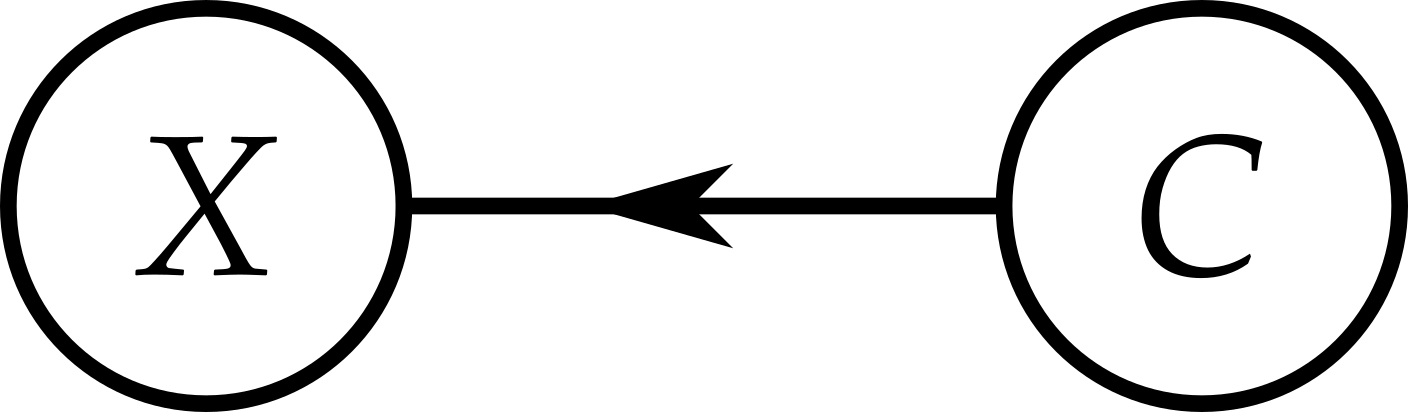
\includegraphics[scale=0.5]{bayesnet1.png}
\end{center}% bayesnet.svg
The two nodes represent the two sets of statements. The arrow from the
$C$-node to the $X$-node represent the conditional exchangeability of the
probabilities for the latter set of statements conditional on the former
set. The absence of incoming arrows to the $C$-node represents the full
exchangeability for its probability distribution. The final integral
representation for the joint probability of full network has a factorizable
density, with one factor per node.

Using the reasoning and integral representations of
\sects~\ref{sec:partial_exch}--\ref{sec:result} it is indeed possible to
generalize these rules to more complex networks of statements. The
following network, for example:
\begin{center}%[h!]
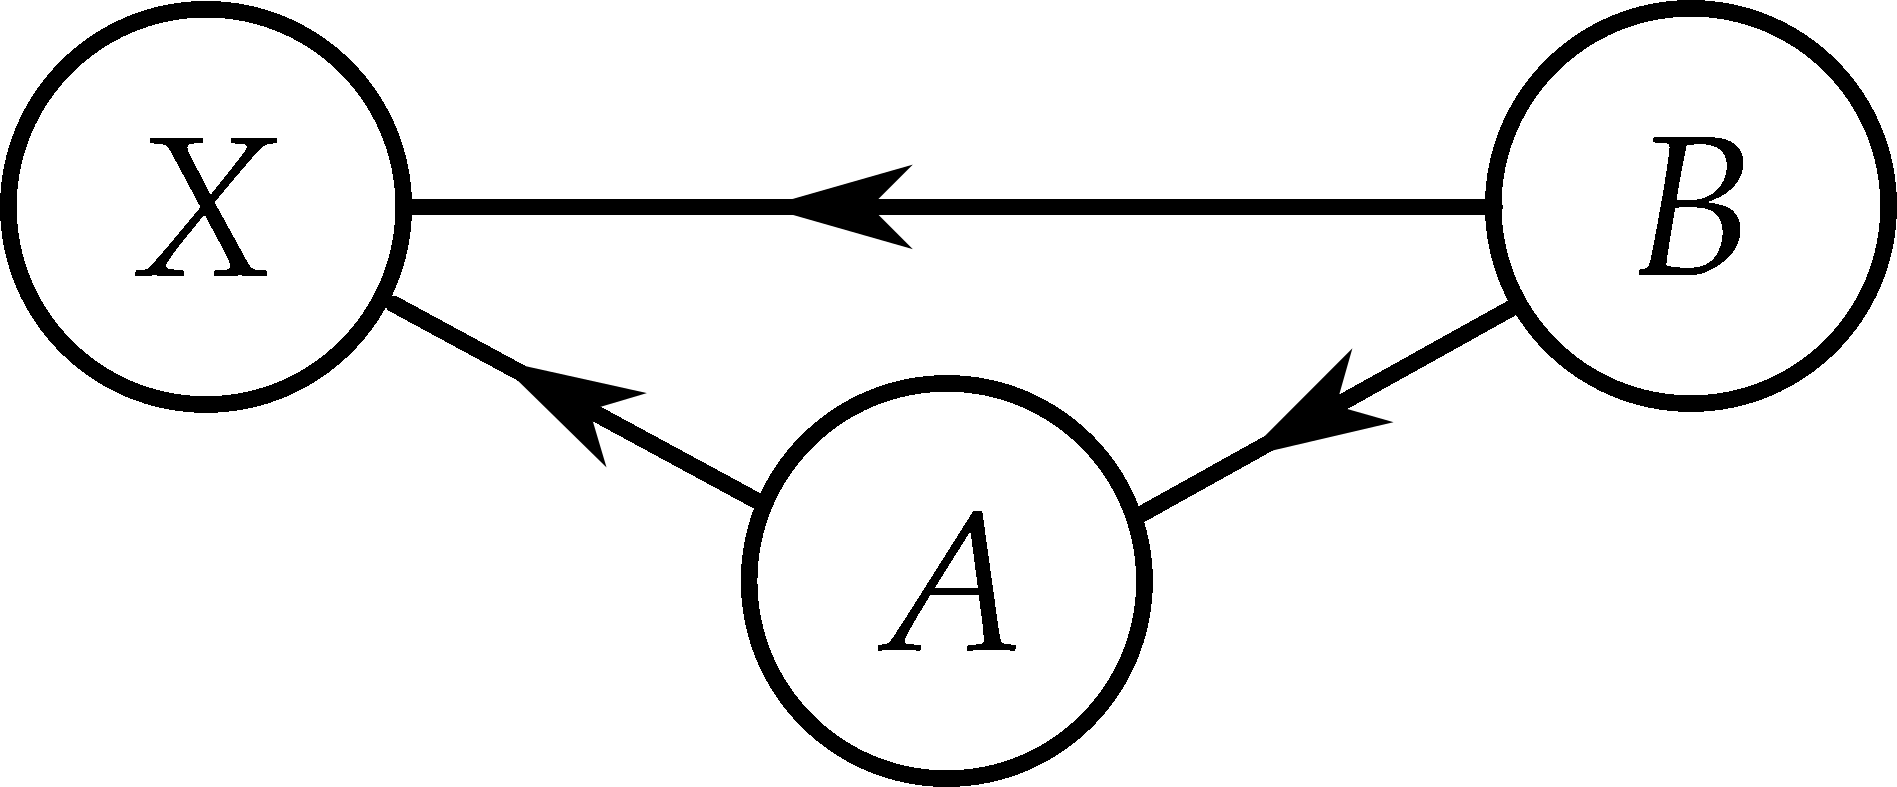
\includegraphics[scale=0.5]{bayesnet3.png}
\end{center}% bayesnet.svg
has the representation
\begin{multline}
  \label{eq:example1}
  \p( \X{1}\=\x{1}, \A{1}\=\va{1}, \B{1}\=\vb{1},\, \dotsc,\,
   \X{N}\=\x{N}, \A{N}\=\va{N}, \B{N}\=\vb{N} \| I) ={}\\
\int\!\prod_{x,a,b} {\ff{x,a,b}}^{N \FF{x,a,b}}\;
\pf(\ffb{x \bcond ab}\|I)\,\pf(\ffb{a \bcond b}\|I)\,\pf(\ffb{b}\|I)
\;\di\ffb{x \bcond ab} \,\di\ffb{a \bcond b} \,\di\ffb{b} \;.
\end{multline}


\subsection{Additional independence assumptions}
\label{sec:graph_repr_indep}

In the last two examples the joint probability density for all the
statements is decomposed in full accord with the product rule. For example,
\begin{multline}
  \label{eq:example_usual_factorization}
  \p( \set{\X{i}\=\x{i}}, \set{\A{i}\=\va{i}}, \set{\B{i}\=\vb{i}} \| I)
  \equiv{}\\
  \p( \set{\X{i}\=\x{i}} \| \set{\A{i}\=\va{i}}, \set{\B{i}\=\vb{i}},\, I)
  \times{}\\
  \p(\set{\A{i}\=\va{i}} \| \set{\B{i}\=\vb{i}},\, I)
\times \p(  \set{\B{i}\=\vb{i}}\| I) \;,
\end{multline}
which is an identity in the probability-calculus. In other words, no
special properties of conditional independence hold. In this case the
integral representation involves an integration over a set of conditional
or marginal long-run frequencies which is equivalent to the set of joint
frequencies. For example, in the representation~\eqref{eq:example1} the
two sets
\begin{equation}
  \label{eq:sets_corr}
  \set{\ff{x \bcond a,b},\, \ff{,a \bcond b},\, \ff{,,b} \|
 x \in \sX, a \in \sA, b \in \sB}
\leftrightarrow
\set{\ff{x,a,b} \| x \in \sX, a \in \sA, b \in \sB}
\end{equation}
are in one-one correspondence.

The factorizability of the density therefore only implies, and is implied
by, the exchangeability symmetries of conditional probability
distributions. It does not imply additional independences.

Additional independence properties, such as
\begin{multline}
  \label{eq:example_independence}
  \p( \set{\X{i}\=\x{i}}, \set{\A{i}\=\va{i}}, \set{\B{i}\=\vb{i}} \| I)
={}\\
  \p( \set{\X{i}\=\x{i}} \| \set{\A{i}\=\va{i}}, \set{\B{i}\=\vb{i}},\, I)
  \times{}\\
  \p(\set{\A{i}\=\va{i}} \|  I)
  \times \p(  \set{\B{i}\=\vb{i}}\| I) \;,
\end{multline}
which is not an identity of the probability-calculus, are instead expressed
by a reduction in the number of conditional or marginal long-run
frequencies in the representation (similarly to what happens when partial
exchangeability reduces to full exchangeability; see
\sect~\ref{sec:partial_exch}).

For example, when the independence~\eqref{eq:example_independence} hold,
the representation~\eqref{eq:example1} becomes
\begin{multline}
  \label{eq:example1sep}
  \p( \X{1}\=\x{1}, \A{1}\=\va{1}, \B{1}\=\vb{1},\, \dotsc,\,
   \X{N}\=\x{N}, \A{N}\=\va{N}, \B{N}\=\vb{N} \| I) ={}\\
   %\shoveleft{
     \int\!\prod_{x,a,b}
     (\ff{x \bcond a,b}\, \ff{,a}\, \ff{,,b})^{N \FF{x,a,b}}\;%\times{}%}\\[-\jot]
\pf(\ffb{x \bcond ab}\|I)\,\pf(\ffb{a}\|I)\,\pf(\ffb{b}\|I)
\;\di\ffb{x \bcond ab} \,\di\ffb{a} \,\di\ffb{b}
\end{multline}
with $\ff{,a} \defd \sum_{x,b}\ff{x,a,b}$ and so on. We see that the
integration is now over the reduced set of long-run distributions
\begin{equation}
  \label{eq:subset_freqs}
  \set{\ff{x \bcond a,b},\, \ff{,a},\, \ff{,,b} \|
    x \in \sX, a \in \sA, b \in \sB} \;.
\end{equation}
Equivalently this reduction can be expressed as
$\ff{,a \bcond b} = \ff{,,a}$ for all $b$, implying the presence of a delta
term in the corresponding density.

The independence condition~\eqref{eq:example_independence} and
integral representation~\eqref{eq:example1sep} can be expressed by the network
\begin{center}%[h!]
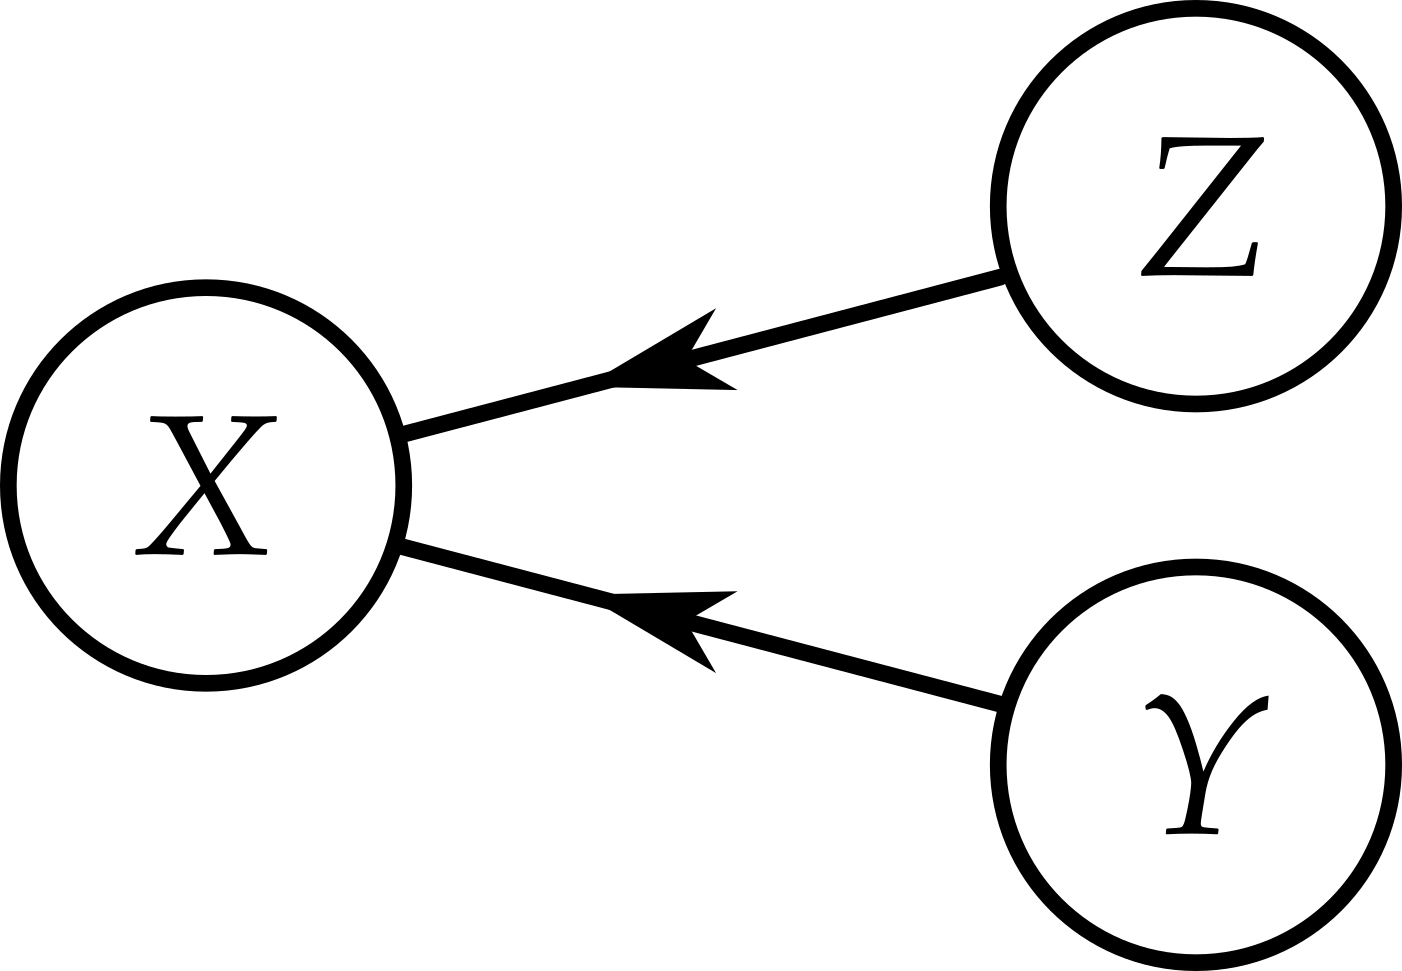
\includegraphics[scale=0.5]{bayesnet3s.png}
\end{center}% bayesnet.svg

\subsection{Generalization and possible graphical rules}
\label{sec:graph_repr_gen}

It seems possible to generalize the example presented thus far into a
consistent set of rules.

We have
\begin{enumerate}[label=\roman*.]
\item several sets of $N$ statements, $\set{\X{i}\=\x{i}}$,
  $\set{\A{i}\=\va{i}},\dotsc$. To each set is associated a set of values
  $x\in \sX,$ $a \in \sA, \dotsc$.
\item several conditionally exchangeable probabilities for some groups of
  such statements conditional on some other groups, such as
  \eqn~\eqref{eq:partial_definetti_freq};
\item several assumptions of conditional independence, such as
  \eqn~\eqref{eq:example_independence}.
\end{enumerate}

The integral representation of the joint probability distribution for all
the statements involves several sets of integration variables. Each set
contains either conditional or marginal long-run frequencies in the
quantities $x,a, \dotsc$.

-- and a factorizable density
over such variables. The density is multiplied by the product of these
variables, raised to the joint empirical frequencies


can then be represented by an acyclic directed network with
these properties:
\begin{enumerate}
\item nodes represent sets of statements;
\item there is a set of integration variables for each node. These
  variables are the long-run frequencies for the quantity of the node
  conditional on the quantities of the parent nodes. Nodes without parents
  have marginal, unconditional long-run frequencies;
\item each set of integration variables has its own density. The densities
  are multiplied in the integral representation.
\end{enumerate}

Moreover, s explained in \sect~\ref{sec:graph_repr_indep}, independence
assumptions are expressed by the set of integration variables, whereas
conditional-exchangeability assumption are expressed by the factorization
of the density over the integration variables.


indicates the conditional exchangeability of the latter set conditional on
the former set. Nodes with no incoming arrows are fully exchangeable. The
integral representation for the full network, that is, for the all the
statements, has a factorizable density, one factor per node. The arguments
of these factors are conditional or marginal long-run frequencies
accordingly to the arrows incoming to their nodes.


\section{Discussion}
\label{sec:discuss}

*** first result can be useful for infinite limits, leading to regression


The result of the previous section is thus summarized: Given infinitely
countable sets of statements $\set{\X{i}\=\x{i}}$ and
$\set{\C{i}\=\cc{i}}$, and assuming that
\begin{enumerate}[wide]
\item the marginal probability distribution for the $C$ statements is fully
  exchangeable,
\item the probability distribution for the $X$ statements is partially (or
  conditionally) exchangeable given the $C$,
\end{enumerate}
Then the joint distribution for both sets is fully exchangeable, and the
density within its integral representation \emph{factorizes} into a density
for a conditional long-run frequency distribution, and a density for a
marginal long-run frequency distribution, \eqn~\eqref{eq:factorizable}.


%%%% examples use empheq
%   \begin{empheq}[left={\mathllap{\begin{aligned}    \de\yF_{\yc}/\de\yp&=0\text{:} \\
%         \de\yF_{\yc}/\de\ym&=0\text{:}\\ \de\yF_{\yc}/\de\yl&=0\text{:}\end{aligned}}\qquad}\empheqlbrace]{align}
%     \label{eq:con_p}
% %    \de\yF_{\yc}/\de\yp &\equiv
%     -\ln\yp + \ln\yq + \yl\yM + \ym\yu &=0,\\
%     \label{eq:con_u}
% %    \de\yF_{\yc}/\de\ym &\equiv
%     \yu\yp-1 &=0,\\
%     \label{eq:con_l}
%     %\de\yF_{\yc}/\de\yl &\equiv
%     \yM\yp-\yc &=0.
%   \end{empheq}
%%%%
% \begin{empheq}[box=\widefbox]{equation}
%   \label{eq:maxent_question}
%   \p\bigl[\yE{N+1}{k} \bigcond \tsum\yo\yf{N}\in\yA, \yM\bigr] = \mathord{?}
% \end{empheq}



% \[
%   \begin{tikzcd}
%       M_{n,n}(\CC) \arrow{r}{R'_{a}(\Hat{U})} & M_{n,n}(\CC)
%     \\
%     L(\mathcal{H}) \arrow{r}{\Hat{U}} \arrow[swap]{d}{R_*}\arrow[swap]{u}{R'_*} & L(\mathcal{H}) \arrow{d}{R_*}\arrow{u}{R'_*} \\
%       M_{n,n}(\CC) \arrow{r}{R_{a}(\Hat{U})} & M_{n,n}(\CC)
%   \end{tikzcd}
% \]

% \[
%   \begin{tikzcd}
%       \CC^n \arrow{r}{R'_*(A)} & \CC^n
%     \\
%     \mathcal{H} \arrow{r}{A} \arrow[swap]{d}{R}\arrow[swap]{u}{R'} & \mathcal{H} \arrow{d}{R}\arrow{u}{R'} \\
%       \CC^n \arrow{r}{R_*(A)} & \CC^n
%   \end{tikzcd}
% \]


% \[
%   \begin{tikzcd}
%     \mathcal{H} \arrow{r}{A} \arrow[swap]{d}{R} & \mathcal{H} \arrow{d}{R} \\
%       \CC^n \arrow{r}{R_*(A)} & \CC^n
%   \end{tikzcd}
% \]

%%\setlength{\intextsep}{0ex}% with wrapfigure
%%\setlength{\columnsep}{0ex}% with wrapfigure
%\begin{figure}[p!]% with figure
%\begin{wrapfigure}{r}{0.4\linewidth} % with wrapfigure
%  \centering\includegraphics[trim={12ex 0 18ex 0},clip,width=\linewidth]{maxent_saddle.png}\\
%\caption{caption}\label{fig:comparison_a5}
%\end{figure}% exp_family_maxent.nb


%%%%%%%%%%%%%%%%%%%%%%%%%%%%%%%%%%%%%%%%%%%%%%%%%%%%%%%%%%%%%%%%%%%%%%%%%%%%
%%% Acknowledgements
%%%%%%%%%%%%%%%%%%%%%%%%%%%%%%%%%%%%%%%%%%%%%%%%%%%%%%%%%%%%%%%%%%%%%%%%%%%% 
\iffalse
\begin{acknowledgements}
  \ldots to Mari \amp\ Miri for continuous encouragement and affection, and
  to Buster Keaton and Saitama for filling life with awe and inspiration.
  To the developers and maintainers of \LaTeX, Emacs, AUC\TeX, Open Science
  Framework, R, Python, Inkscape, Sci-Hub for making a free and impartial
  scientific exchange possible.
%\rotatebox{15}{P}\rotatebox{5}{I}\rotatebox{-10}{P}\rotatebox{10}{\reflectbox{P}}\rotatebox{-5}{O}.
%\sourceatright{\autanet}
\mbox{}\hfill\autanet
\end{acknowledgements}
\fi

%%%%%%%%%%%%%%%%%%%%%%%%%%%%%%%%%%%%%%%%%%%%%%%%%%%%%%%%%%%%%%%%%%%%%%%%%%%%
%%% Appendices
%%%%%%%%%%%%%%%%%%%%%%%%%%%%%%%%%%%%%%%%%%%%%%%%%%%%%%%%%%%%%%%%%%%%%%%%%%%% 
\clearpage
% %\renewcommand*{\appendixpagename}{Appendix}
% %\renewcommand*{\appendixname}{Appendix}
% %\appendixpage
% \appendix

%%%%%%%%%%%%%%%%%%%%%%%%%%%%%%%%%%%%%%%%%%%%%%%%%%%%%%%%%%%%%%%%%%%%%%%%%%%%
%%% Bibliography
%%%%%%%%%%%%%%%%%%%%%%%%%%%%%%%%%%%%%%%%%%%%%%%%%%%%%%%%%%%%%%%%%%%%%%%%%%%% 
\renewcommand*{\finalnamedelim}{\addcomma\space}
\defbibnote{prenote}{{\footnotesize (\enquote{de $X$} is listed under D,
    \enquote{van $X$} under V, and so on, regardless of national
    conventions.)\par}}
% \defbibnote{postnote}{\par\medskip\noindent{\footnotesize% Note:
%     \arxivp \mparcp \philscip \biorxivp}}

\printbibliography[prenote=prenote%,postnote=postnote
]

\end{document}

%%%%%%%%%%%%%%%%%%%%%%%%%%%%%%%%%%%%%%%%%%%%%%%%%%%%%%%%%%%%%%%%%%%%%%%%%%%%
%%% Cut text (won't be compiled)
%%%%%%%%%%%%%%%%%%%%%%%%%%%%%%%%%%%%%%%%%%%%%%%%%%%%%%%%%%%%%%%%%%%%%%%%%%%% 




Leaving for the moment
the definition of symbols to intuition, the theorem rewrites a joint
probability distribution as a law of total probability:
\begin{equation}
  \label{eq:definetti}
  \p( \X{1}\=\x{1},\; \X{2}\=\x{2},\; \dotsc \| \zI) =
  \int
  \prod_{i} f_{\x{i}}\;
  \pf(\fx \| \zI)\,\di\fx \;,
\end{equation}
where $\fx \defd (f_{x})$ is a distribution over the values that can be
assumed by each quantity $\X{i}$, and the integral is over the simplex of
such distributions.

The condition for the theorem to hold is that the joint distribution be
infinitely \emph{fully exchangeable}, that is, symmetric with respect to
permutations of the $\x{i}$, for any set of indices $\set{i}$. This formula
is the infinite limit of the sampling formula from an urn of unknown
content. From now on \enquote{exchangeable} shall be understood as
\enquote{infinitely exchangeable}.

A more general version of the theorem holds if the joint distribution is
\emph{partially exchangeable}, that is, if the set $\set{\X{i}}$ is divided
into two or more categories represented by subsets
$\set{\Y{j}}, \set{\Z{k}}, \dotsc$, and permutations are allowed within
each subset but not necessarily across subsets. The formula then becomes,
with a suitable re-indexing
$\set{1,2,\dotsc} \mapsto \set{1', 2', \dotsc, 1'', 2'', \dotsc}$,
\begin{multline}
  \label{eq:partialdefinetti}
  \p( \Y{1'}\=\y{1'},\; \Y{2'}\=\y{2'},\; \dotsc,\;
  \Z{1''}\=\z{1''},\; \Z{2''}\=\z{2''},\; \dotsc \| \zI) ={}\\
  \iint
  \prod_{j} g_{\y{j}}\;
  \prod_{k} h_{\z{k}}\;
  \pf(\bg,\bh \| \zI)\,\di\bg\,\di\bh \;,
\end{multline}
with distinct distributions $\bg$, $\bh$ for each category. If the density
$\pf(\bg,\bh \| \zI)\,\di\bg\,\di\bh$ is diagonal, that is, if it contains
a term $\delt(\bg-\bh)$, the fully exchangeable form~\eqref{eq:definetti}
is recovered.



With a little reflection we see that if we know that the quantities $X$
belong to category $Y$ in instances $1',2',\dotsc$, and to category $Z$ in
instances $1'',2'',\dotsc$, then
\begin{enumerate*}[label=(\alph*)]
\item there is some other quantity $C$ that allows us to distinguish the
  two categories, and \item the values $\C{i}\=\cc{i}$ of this quantity
  \emph{are known} for all instances.
\end{enumerate*}

Let us say, for example, that the quantities $\X{i}$ are the results of
animal treatments, with values \enquote{$\xs$}uccess and
\enquote{$\xf$}ailure. $Y$ refers to the results for treatments on
$\xY$aks, and $Z$ on $\xZ$ebras. If we write
$$\p(\Y{3}\=\xs,\;\Z{5}\=\xf \| \zI)=0.2\;,$$
then we must already know that animal number~$3$ is a yak, $\C{3}\=\xY$,
and animal number~$5$ is a zebra, $\C{5}\=\xZ$. This is clear from our very
notation, otherwise we would not have known whether to use the symbol $Y$
or $Z$ for those instances. This information is evidently implicit in our
background information $\zI$.

Let us make the information about the $\C{i}$ explicit. Their possible
values are \enquote{$\xY$} and \enquote{$\xZ$}. We rewrite the probability
in \eqn~\eqref{eq:partialdefinetti} as
\begin{equation}
  \label{eq:infoCexplicit}
  \begin{aligned}
  &\p( \Y{1'}\=\y{1'},\; %\Y{2'}\=\y{2'},\;
  \dotsc,\;
  \Z{1''}\=\z{1''},\; %\Z{2''}\=\z{2''},\;
  \dotsc \| \zI) \equiv{}\\
  &
\p( \X{1'}\=\x{1'},\; %\X{2'}\=\x{2'},\;
  \dotsc,\;
  \X{1''}\=\x{1''},\; %\X{2''}\=\x{2''},\;
  \dotsc \| %{}\\
  \C{1'}\=\xY,\; %\C{2'}\=\cc{2'},\;
  \dotsc,\;
  \C{1''}\=\xZ,\; %\C{2''}\=\cc{2''},\;
  \dotsc,\; I) \;.
  \end{aligned}
\end{equation}

Then it is clear that the partially exchangeable probability
distribution~\eqref{eq:partialdefinetti} or \eqref{eq:infoCexplicit} can
also be called \emph{conditionally exchangeable}.




The present work gives a representation formula for pairs of quantities
$(\X{i},\C{i})$ such that
\begin{enumerate}%[nosep]
\item the distribution for the $\set{\X{i}}$ is conditionally exchangeable,
  given $\set{\C{i}}$,
\item the distribution for the $\set{\C{i}}$ is fully exchangeable.
\end{enumerate}
The formula is:
%\begin{empheq}{equation}
\begin{subequations}
  \label{eq:result}
  \begin{gather}
  \p\bigl[ (\X{1}\eq\x{1}, \C{1}\eq\cc{1}),\;
  (\X{2}\eq\x{2}, \C{2}\eq\cc{2}),\; \dotsc \| I \bigr] =
 \int \prod_{i}f_{\x{i},\cc{i}}\;
  \pf(\fx\|I)\,\di\fx\\
  \label{eq:factorizable}
\text{with}\qquad \boxed{\;\vphantom{\int}\pf(\fx\|I)\,\di\fx =
  \pf[(f_{x \bcond c}) \|I]\,\di(f_{x \bcond c})
  \times
  \pf[(f_{,c}) \|I]\,\di(f_{,c})\;}
\end{gather}
\end{subequations}
%\end{empheq}%\\[-2\baselineskip]
where
\begin{itemize}%[label=\textendash]
\item $\fx \defd (f_{x, c})$ is a joint distribution over the set of values
  that can be assumed by each $(\X{i},\C{i})$ pair,
\item $\bigl(f_{,c} \defd \sum_{x}f_{x, c} \bigr)$ is the related
  \emph{marginal} frequency distribution for the $c$ values,
\item $\bigl(f_{x \bcond c} \defd f_{x, c}/f_{,c} \bigr)$ are the related
  \emph{conditional} frequency distributions of $x$ given $c$.
\end{itemize}



The formula~\eqref{eq:result} shows that the pairs $(\X{i},\C{i})$ have a
fully exchangeable distribution, with a representation analogous to
\eqn~\eqref{eq:definetti}. The noteworthy feature of this formula is that
\emph{the density $\pf(\fx\|I)\,\di\fx$ is factorizable into the product of
  a density for the conditional frequencies $(f_{x \bcond c})$ and a
  density for the marginal frequencies $(f_{,c})$}, according to
\eqn~\eqref{eq:factorizable}. This factorization expresses the conditional
exchangeability for $\set{\X{i}}$ given $\set{\C{i}}$.



The proof of formula is given in the next section. In the final section I
discuss possible generalizations and connections with Bayesian belief
networks.



%%% Local Variables: 
%%% mode: LaTeX
%%% TeX-PDF-mode: t
%%% TeX-master: t
%%% End: 
